\documentclass[a4paper, 12pt, oneside, openary]{jbook}
%\usepackage[dvipdfmx]{graphicx}
\setlength{\textwidth}{470pt}
\setlength{\topmargin}{-2truemm}
\setlength{\textheight}{650pt}
\setlength{\oddsidemargin}{-0.4truemm}
\setlength{\evensidemargin}{-0.4truemm}


%%%%%%%%%%%%
% 	 UsePackege	%
%%%%%%%%%%%%
\usepackage{amssymb}
\usepackage{amsmath}
\usepackage{amsthm}
\usepackage{ascmac}
\usepackage{lscape}
\usepackage{pifont}
\usepackage{cite}
\usepackage{ifthen}
\usepackage{framed}
\usepackage{mathrsfs}
\usepackage{booktabs}
\usepackage{algorithm}
\usepackage{algorithmic}
\usepackage{comment}
\usepackage{longtable}
% Font
%%%%%%%%%%%%%%
% 	Bold Number	%
%%%%%%%%%%%%%%
\newcommand{\bzero}{{\bf 0}}
\newcommand{\bone}{{\bf 1}}
%%%%%%%%%%%%%%
% 	Bold English	%
%%%%%%%%%%%%%%
% a
\newcommand{\ba}{{\mbox{\boldmath$a$}}}
\newcommand{\bA}{{\mbox{\boldmath$A$}}}
\newcommand{\sba}{{\mbox{\scriptsize\boldmath $a$}}}
% b
\newcommand{\bb}{{\mbox{\boldmath$b$}}}
\newcommand{\bB}{{\mbox{\boldmath$B$}}}
\newcommand{\sbb}{{\mbox{\scriptsize\boldmath $b$}}}
% c
\newcommand{\bc}{{\mbox{\boldmath$c$}}}
\newcommand{\bC}{{\mbox{\boldmath$C$}}}
\newcommand{\sbC}{{\mbox{\scriptsize\boldmath $C$}}}
\newcommand{\sbc}{{\mbox{\scriptsize\boldmath $c$}}}
% d
\newcommand{\bd}{{\mbox{\boldmath$d$}}}
\newcommand{\bD}{{\mbox{\boldmath$D$}}}
\newcommand{\sbd}{{\mbox{\scriptsize\boldmath $d$}}}
% e
\newcommand{\be}{{\mbox{\boldmath$e$}}}
\newcommand{\bE}{{\mbox{\boldmath$E$}}}
\newcommand{\sbe}{{\mbox{\scriptsize\boldmath $e$}}}
% f
\newcommand{\bbf}{{\mbox{\boldmath$f$}}}
\newcommand{\bF}{{\mbox{\boldmath$F$}}}
% g
\newcommand{\bg}{{\mbox{\boldmath$g$}}}
\newcommand{\bG}{{\mbox{\boldmath$G$}}}
% h
\newcommand{\bh}{{\mbox{\boldmath$h$}}}
\newcommand{\bH}{{\mbox{\boldmath$H$}}}
\newcommand{\sbH}{{\mbox{\scriptsize\boldmath$H$}}}
\newcommand{\sbh}{{\mbox{\scriptsize\boldmath$h$}}}
% i
\newcommand{\bi}{{\mbox{\boldmath$i$}}}
\newcommand{\sbi}{{\mbox{\scriptsize \boldmath$i$}}}
\newcommand{\bI}{{\mbox{\boldmath$I$}}}
% i
\newcommand{\bj}{{\mbox{\boldmath$j$}}}
\newcommand{\sbj}{{\mbox{\scriptsize \boldmath$j$}}}
\newcommand{\bJ}{{\mbox{\boldmath$J$}}}
% k
\newcommand{\bk}{{\mbox{\boldmath$k$}}}
\newcommand{\bK}{{\mbox{\boldmath$K$}}}
% l
%\newcommand{\ell}{{\mbox{\boldmath $l$}}}
\newcommand{\bl}{{\mbox{\boldmath$l$}}}
\newcommand{\bL}{{\mbox{\boldmath$L$}}}
% m
\newcommand{\bm}{{\mbox{\boldmath$m$}}}
\newcommand{\sbm}{{\mbox{\scriptsize \boldmath$m$}}}
\newcommand{\bM}{{\mbox{\boldmath$M$}}}
% n
\newcommand{\bn}{{\mbox{\boldmath$n$}}}
\newcommand{\bN}{{\mbox{\boldmath$N$}}}
\newcommand{\sbn}{{\mbox{\scriptsize \boldmath$n$}}}
\newcommand{\sbN}{{\mbox{\scriptsize\boldmath $N$}}}
% o
\newcommand{\bo}{{\mbox{\boldmath$o$}}}
\newcommand{\bO}{{\mbox{\boldmath$O$}}}
% p
\newcommand{\bp}{{\mbox{\boldmath$p$}}}
\newcommand{\bP}{{\mbox{\boldmath$P$}}}
\newcommand{\sbp}{{\mbox{\scriptsize \boldmath$p$}}}
% q
\newcommand{\bq}{{\mbox{\boldmath$q$}}}
\newcommand{\bQ}{{\mbox{\boldmath$Q$}}}
% r
\newcommand{\br}{{\mbox{\boldmath$r$}}}
\newcommand{\bR}{{\mbox{\boldmath$R$}}}
\newcommand{\sbr}{{\mbox{\scriptsize\boldmath$r$}}}
% s
\newcommand{\bs}{{\mbox{\boldmath$s$}}}
\newcommand{\sbs}{{\mbox{\scriptsize \boldmath$s$}}}
\newcommand{\bS}{{\mbox{\boldmath$S$}}}
% t
\newcommand{\bt}{{\mbox{\boldmath$t$}}}
\newcommand{\bT}{{\mbox{\boldmath$T$}}}
% u
\newcommand{\bu}{{\mbox{\boldmath$u$}}}
\newcommand{\bU}{{\mbox{\boldmath$U$}}}
\newcommand{\sbu}{{\mbox{\scriptsize\boldmath $u$}}}
% v
\newcommand{\bv}{{\mbox{\boldmath$v$}}}
\newcommand{\bV}{{\mbox{\boldmath$V$}}}
\newcommand{\sbv}{{\mbox{\scriptsize\boldmath $v$}}}
\newcommand{\sbV}{{\mbox{\scriptsize\boldmath $V$}}}
% w
\newcommand{\bw}{{\mbox{\boldmath$w$}}}
\newcommand{\bW}{{\mbox{\boldmath$W$}}}
\newcommand{\sbW}{{\mbox{\scriptsize\boldmath $W$}}}
\newcommand{\sbw}{{\mbox{\scriptsize\boldmath $w$}}}
% x
\newcommand{\bx}{{\mbox{\boldmath$x$}}}
\newcommand{\bX}{{\mbox{\boldmath$X$}}}
\newcommand{\sbx}{{\mbox{\scriptsize\boldmath $x$}}}
\newcommand{\sbX}{{\mbox{\scriptsize\boldmath $X$}}}
%y
\newcommand{\by}{{\mbox{\boldmath$y$}}}
\newcommand{\bY}{{\mbox{\boldmath$Y$}}}
\newcommand{\sby}{{\mbox{\scriptsize\boldmath $y$}}}
\newcommand{\sbY}{{\mbox{\scriptsize\boldmath $Y$}}}
%z
\newcommand{\bz}{{\mbox{\boldmath$z$}}}
\newcommand{\bZ}{{\mbox{\boldmath$Z$}}}
\newcommand{\sbz}{{\mbox{\scriptsize\boldmath$z$}}}
\newcommand{\sbZ}{{\mbox{\scriptsize\boldmath$Z$}}}


%%%%%%%%%%%
% 	Bold Grik	%
%%%%%%%%%%%
% alpha
\newcommand{\balpha}{{\mbox{\boldmath$\alpha$}}}
\newcommand{\sbalpha}{{\mbox{\scriptsize\boldmath$\alpha$}}}
% beta
\newcommand{\bbeta}{{\mbox{\boldmath$\beta$}}}
\newcommand{\sbbeta}{{\mbox{\scriptsize\boldmath$\beta$}}}
% gamma
\newcommand{\bgamma}{{\mbox{\boldmath$\gamma$}}}
\newcommand{\bGamma}{{\mbox{\boldmath$\Gamma$}}}
\newcommand{\sbgamma}{{\mbox{\scriptsize\boldmath$\gamma$}}}
% delta
\newcommand{\bdelta}{{\mbox{\boldmath$\delta$}}}
\newcommand{\bDelta}{{\mbox{\boldmath$\Delta$}}}
\newcommand{\sbdelta}{{\mbox{\scriptsize\boldmath$\delta$}}}
% epsilon
\newcommand{\bepsilon}{{\mbox{\boldmath$\epsilon$}}}
\newcommand{\bvarepsilon}{{\mbox{\boldmath$\varepsilon$}}}
\newcommand{\sbvarepsilon}{{\mbox{\scriptsize\boldmath$\varepsilon$}}}
% zeta
\newcommand{\bzeta}{{\mbox{\boldmath$\zeta$}}}
% eta
\newcommand{\etab}{{\mbox{\boldmath$\eta$}}}
% theta
\newcommand{\btheta}{{\mbox{\boldmath$\theta$}}}
\newcommand{\bTheta}{{\mbox{\boldmath$\Theta$}}}
\newcommand{\bvartheta}{{\mbox{\boldmath$\vartheta$}}}
\newcommand{\sbtheta}{{\mbox{\scriptsize\boldmath$\theta$}}}
\newcommand{\sbTheta}{{\mbox{\scriptsize\boldmath$\Theta$}}}
% iota
\newcommand{\biota}{{\mbox{\boldmath$\iota$}}}
\newcommand{\sbiota}{{\mbox{\scriptsize\boldmath$\iota$}}}
% kappa
\newcommand{\bkappa}{{\mbox{\boldmath$\kappa$}}}
% lambda
\newcommand{\blambda}{{\mbox{\boldmath$\lambda$}}}
\newcommand{\bLambda}{{\mbox{\boldmath$\Lambda$}}}
% mu
\newcommand{\bmu}{{\mbox{\boldmath$\mu$}}}
\newcommand{\sbmu}{{\mbox{\scriptsize\boldmath$\mu$}}}
% nu
\newcommand{\bnu}{{\mbox{\boldmath$\nu$}}}
\newcommand{\sbnu}{{\mbox{\scriptsize\boldmath$\nu$}}}
% xi
\newcommand{\bxi}{{\mbox{\boldmath$\xi$}}}
\newcommand{\bXi}{{\mbox{\boldmath$\Xi$}}}
% pi
\newcommand{\bpi}{{\mbox{\boldmath$\pi$}}}
\newcommand{\bPi}{{\mbox{\boldmath$\Pi$}}}
\newcommand{\bvarpi}{{\mbox{\boldmath$\varpi$}}}
% rho
\newcommand{\brho}{{\mbox{\boldmath$\rho$}}}
\newcommand{\bvarrho}{{\mbox{\boldmath$\varrho$}}}
% sigma
\newcommand{\bsigma}{{\mbox{\boldmath$\sigma$}}}
\newcommand{\bSigma}{{\mbox{\boldmath$\Sigma$}}}
\newcommand{\bvarsigma}{{\mbox{\boldmath$\varsigma$}}}
% tau
\newcommand{\btau}{{\mbox{\boldmath$\tau$}}}
% upsilon
\newcommand{\bupsilon}{{\mbox{\boldmath$\upsilon$}}}
\newcommand{\bUpsilon}{{\mbox{\boldmath$\Upsilon$}}}
% phi
\newcommand{\bphi}{{\mbox{\boldmath$\phi$}}}
\newcommand{\bPhi}{\mathbf \Phi}
\newcommand{\bvarphi}{{\mbox{\boldmath$\varphi$}}}
% chi
\newcommand{\bchi}{{\mbox{\boldmath$\chi$}}}
% psi
\newcommand{\bpsi}{{\mbox{\boldmath$\psi$}}}
\newcommand{\bPsi}{\mathbf \Psi}
% omega
\newcommand{\bomega}{{\mbox{\boldmath$\omega$}}}
\newcommand{\bOmega}{{\mbox{\boldmath$\Omega$}}}
% nabla
\newcommand{\bnabla}{{\mbox{\boldmath$\nabla$}}}

% calligraphic letters
\newcommand{\cA}{{\cal A}}
\newcommand{\cB}{{\cal B}}
\newcommand{\cC}{{\cal C}}
\newcommand{\cD}{{\cal D}}
\newcommand{\cE}{{\cal E}}
\newcommand{\cF}{{\cal F}}
\newcommand{\cG}{{\cal G}}
\newcommand{\cH}{{\cal H}}
\newcommand{\cI}{{\cal I}}
\newcommand{\cJ}{{\cal J}}
\newcommand{\cK}{{\cal K}}
\newcommand{\cL}{{\cal L}}
\newcommand{\cM}{{\cal M}}
\newcommand{\cN}{{\cal N}}
\newcommand{\cO}{{\cal O}}
\newcommand{\cP}{{\cal P}}
\newcommand{\cQ}{{\cal Q}}
\newcommand{\cR}{{\cal R}}
\newcommand{\cS}{{\cal S}}
\newcommand{\cT}{{\cal T}}
\newcommand{\cU}{{\cal U}}
\newcommand{\cV}{{\cal V}}
\newcommand{\cW}{{\cal W}}
\newcommand{\cX}{{\cal X}}
\newcommand{\cY}{{\cal Y}}
\newcommand{\cZ}{{\cal Z}}
% calligraphic letters
\newcommand{\mA}{{\mathscr A}}
\newcommand{\mB}{{\mathscr B}}
\newcommand{\mC}{{\mathscr C}}
\newcommand{\mD}{{\mathscr D}}
\newcommand{\mE}{{\mathscr E}}
\newcommand{\mF}{{\mathscr F}}
\newcommand{\mG}{{\mathscr G}}
\newcommand{\mH}{{\mathscr H}}
\newcommand{\mI}{{\mathscr I}}
\newcommand{\mJ}{{\mathscr J}}
\newcommand{\mK}{{\mathscr K}}
\newcommand{\mL}{{\mathscr L}}
\newcommand{\mM}{{\mathscr M}}
\newcommand{\mN}{{\mathscr N}}
\newcommand{\mO}{{\mathscr O}}
\newcommand{\mP}{{\mathscr P}}
\newcommand{\mQ}{{\mathscr Q}}
\newcommand{\mR}{{\mathscr R}}
\newcommand{\mS}{{\mathscr S}}
\newcommand{\mT}{{\mathscr T}}
\newcommand{\mU}{{\mathscr U}}
\newcommand{\mV}{{\mathscr V}}
\newcommand{\mW}{{\mathscr W}}
\newcommand{\mX}{{\mathscr X}}
\newcommand{\mY}{{\mathscr Y}}
\newcommand{\mZ}{{\mathscr Z}}
\input{../../Lab/stylefiles/rules/MyBB}
%%%%%%%%%%%%%%
% 	Tilde English	%
%%%%%%%%%%%%%%
% a
\newcommand{\tila}{\tilde{a}}
\newcommand{\tilA}{\tilde{A}}
% b
\newcommand{\tilb}{\tilde{b}}
\newcommand{\tilB}{\tilde{B}}
% c
\newcommand{\tilc}{\tilde{c}}
\newcommand{\tilC}{\tilde{C}}
% d
\newcommand{\tild}{\tilde{d}}
\newcommand{\tilD}{\tilde{D}}
% e
\newcommand{\tile}{\tilde{e}}
\newcommand{\tilE}{\tilde{E}}
% f
\newcommand{\tilf}{\tilde{f}}
\newcommand{\tilF}{\tilde{F}}
% g
\newcommand{\tilg}{\tilde{g}}
\newcommand{\tilG}{\tilde{G}}
% h
\newcommand{\tilh}{\tilde{h}}
\newcommand{\tilbh}{\tilde\bh}
\newcommand{\tilH}{\tilde{H}}
% i
\newcommand{\tili}{\tilde{i}}
\newcommand{\tilI}{\tilde{I}}
% i
\newcommand{\tilj}{\tilde{j}}
\newcommand{\tilJ}{\tilde{J}}
% k
\newcommand{\tilk}{\tilde{k}}
\newcommand{\tilK}{\tilde{K}}
% l
\newcommand{\till}{\tilde{l}}
\newcommand{\tilL}{\tilde{L}}
% m
\newcommand{\tilm}{\tilde{m}}
\newcommand{\tilM}{\tilde{M}}
% n
\newcommand{\tiln}{\tilde{n}}
\newcommand{\tilN}{\tilde{N}}
% o
\newcommand{\tilo}{\tilde{o}}
\newcommand{\tilO}{\tilde{O}}
% p
\newcommand{\tilp}{\tilde{p}}
\newcommand{\tilP}{\tilde{P}}
% q
\newcommand{\tilq}{\tilde{q}}
\newcommand{\tilQ}{\tilde{Q}}
\newcommand{\tilbq}{\tilde{\bq}}
% r
\newcommand{\tilr}{\tilde{r}}
\newcommand{\tilR}{\tilde{R}}
\newcommand{\tilcR}{\tilde{\cR}}
\newcommand{\tilbr}{\tilde{\br}}
% s
\newcommand{\tils}{\tilde{s}}
\newcommand{\tilS}{\tilde{S}}
% t
\newcommand{\tilt}{\tilde{t}}
\newcommand{\tilT}{\tilde{T}}
% u
\newcommand{\tilu}{\tilde{u}}
\newcommand{\tilU}{\tilde{U}}
% v
\newcommand{\tilv}{\tilde{v}}
\newcommand{\tilV}{\tilde{V}}
% w
\newcommand{\tilw}{\tilde{w}}
\newcommand{\tilW}{\tilde{W}}
% x
\newcommand{\tilx}{\tilde{x}}
\newcommand{\tilbx}{\tilde{\bx}}
\newcommand{\tilX}{\tilde{X}}
\newcommand{\tilbX}{\tilde{\bX}}
%y
\newcommand{\tily}{\tilde{y}}
\newcommand{\tilY}{\tilde{Y}}
\newcommand{\tilby}{\tilde{\by}}
\newcommand{\tilbY}{\tilde{\bY}}
%z
\newcommand{\tilz}{\tilde{z}}
\newcommand{\tilZ}{\tilde{Z}}
\newcommand{\tilbZ}{\tilde{\bZ}}


%%%%%%%%%%%%
%% 	Bold Grik	%
%%%%%%%%%%%%
%% alpha
\newcommand{\tilalpha}{\tilde{\alpha}}
%\newcommand{\sbalpha}{{\mbox{\scriptsize\boldmath$\alpha$}}}
%% beta
\newcommand{\tilbeta}{{\tilde{\beta}}}
%\newcommand{\sbbeta}{{\mbox{\scriptsize\boldmath$\beta$}}}
%% gamma
\newcommand{\tilgamma}{{\tilde{\gamma}}}
%\newcommand{\bGamma}{{\mbox{\boldmath$\Gamma$}}}
%\newcommand{\sbgamma}{{\mbox{\scriptsize\boldmath$\gamma$}}}
%% delta
%\newcommand{\bdelta}{{\mbox{\boldmath$\delta$}}}
%\newcommand{\bDelta}{{\mbox{\boldmath$\Delta$}}}
%\newcommand{\sbdelta}{{\mbox{\scriptsize\boldmath$\delta$}}}
%% epsilon
%\newcommand{\bepsilon}{{\mbox{\boldmath$\epsilon$}}}
%\newcommand{\bvarepsilon}{{\mbox{\boldmath$\varepsilon$}}}
%\newcommand{\sbvarepsilon}{{\mbox{\scriptsize\boldmath$\varepsilon$}}}
%% zeta
%\newcommand{\bzeta}{{\mbox{\boldmath$\zeta$}}}
%% eta
%\newcommand{\etab}{{\mbox{\boldmath$\eta$}}}
%% theta
%\newcommand{\btheta}{{\mbox{\boldmath$\theta$}}}
%\newcommand{\bTheta}{{\mbox{\boldmath$\Theta$}}}
%\newcommand{\bvartheta}{{\mbox{\boldmath$\vartheta$}}}
%% iota
%\newcommand{\biota}{{\mbox{\boldmath$\iota$}}}
%\newcommand{\sbiota}{{\mbox{\scriptsize\boldmath$\iota$}}}
%% kappa
%\newcommand{\bkappa}{{\mbox{\boldmath$\kappa$}}}
%% lambda
%\newcommand{\blambda}{{\mbox{\boldmath$\lambda$}}}
%\newcommand{\bLambda}{{\mbox{\boldmath$\Lambda$}}}
%% mu
%\newcommand{\bmu}{{\mbox{\boldmath$\mu$}}}
%\newcommand{\sbmu}{{\mbox{\scriptsize\boldmath$\mu$}}}
%% nu
%\newcommand{\bnu}{{\mbox{\boldmath$\nu$}}}
%\newcommand{\sbnu}{{\mbox{\scriptsize\boldmath$\nu$}}}
%% xi
%\newcommand{\bxi}{{\mbox{\boldmath$\xi$}}}
%\newcommand{\bXi}{{\mbox{\boldmath$\Xi$}}}
%% pi
%\newcommand{\bpi}{{\mbox{\boldmath$\pi$}}}
%\newcommand{\bPi}{{\mbox{\boldmath$\Pi$}}}
%\newcommand{\bvarpi}{{\mbox{\boldmath$\varpi$}}}
%% rho
%\newcommand{\brho}{{\mbox{\boldmath$\rho$}}}
%\newcommand{\bvarrho}{{\mbox{\boldmath$\varrho$}}}
%% sigma
%\newcommand{\bsigma}{{\mbox{\boldmath$\sigma$}}}
%\newcommand{\bSigma}{{\mbox{\boldmath$\Sigma$}}}
%\newcommand{\bvarsigma}{{\mbox{\boldmath$\varsigma$}}}
% tau
\newcommand{\tiltau}{{\mbox{$\tilde{\tau}$}}}
%% upsilon
%\newcommand{\bupsilon}{{\mbox{\boldmath$\upsilon$}}}
%\newcommand{\bUpsilon}{{\mbox{\boldmath$\Upsilon$}}}
%% phi
%\newcommand{\bphi}{{\mbox{\boldmath$\phi$}}}
%\newcommand{\bPhi}{\mathbf \Phi}
%\newcommand{\bvarphi}{{\mbox{\boldmath$\varphi$}}}
%% chi
%\newcommand{\bchi}{{\mbox{\boldmath$\chi$}}}
%% psi
%\newcommand{\bpsi}{{\mbox{\boldmath$\psi$}}}
%\newcommand{\bPsi}{\mathbf \Psi}
%% omega
%\newcommand{\bomega}{{\mbox{\boldmath$\omega$}}}
%\newcommand{\bOmega}{{\mbox{\boldmath$\Omega$}}}

%%%%%%%%%%%%%%
% 	Tilde English	%
%%%%%%%%%%%%%%
% a
\newcommand{\bara}{\bar{a}}
\newcommand{\barA}{\bar{A}}
% b
\newcommand{\barb}{\bar{b}}
\newcommand{\barB}{\bar{B}}
% c
\newcommand{\barc}{\bar{c}}
\newcommand{\barC}{\bar{C}}
% d
\newcommand{\bard}{\bar{d}}
\newcommand{\barD}{\bar{D}}
% e
\newcommand{\bare}{\bar{e}}
\newcommand{\barE}{\bar{E}}
% f
\newcommand{\barbf}{\bar{f}}
\newcommand{\barF}{\bar{F}}
% g
\newcommand{\barg}{\bar{g}}
\newcommand{\barG}{\bar{G}}
% h
\newcommand{\barh}{\bar{h}}
\newcommand{\barbh}{\bar\bh}
\newcommand{\barH}{\bar{H}}
% i
\newcommand{\bari}{\bar{i}}
\newcommand{\barI}{\bar{I}}
% i
\newcommand{\barj}{\bar{j}}
\newcommand{\barJ}{\bar{J}}
% k
\newcommand{\bark}{\bar{k}}
\newcommand{\barK}{\bar{K}}
% l
\newcommand{\barl}{\bar{l}}
\newcommand{\barL}{\bar{L}}
% m
\newcommand{\barm}{\bar{m}}
\newcommand{\barM}{\bar{M}}
% n
\newcommand{\barn}{\bar{n}}
\newcommand{\barN}{\bar{N}}
% o
\newcommand{\baro}{\bar{o}}
\newcommand{\barO}{\bar{O}}
% p
\newcommand{\barp}{\bar{p}}
\newcommand{\barP}{\bar{P}}
% q
\newcommand{\barq}{\bar{q}}
\newcommand{\barQ}{\bar{Q}}
% r
\newcommand{\barr}{\bar{r}}
\newcommand{\barR}{\bar{R}}
% s
\newcommand{\bars}{\bar{s}}
\newcommand{\barS}{\bar{S}}
% t
\newcommand{\bart}{\bar{t}}
\newcommand{\barT}{\bar{T}}
% u
\newcommand{\baru}{\bar{u}}
\newcommand{\barU}{\bar{U}}
% v
\newcommand{\barv}{\bar{v}}
\newcommand{\barV}{\bar{V}}
% w
\newcommand{\barw}{\bar{w}}
\newcommand{\barW}{\bar{W}}
\newcommand{\barbw}{\bar{\bw}}
% x
\newcommand{\barx}{\bar{x}}
\newcommand{\barX}{\bar{X}}
%y
\newcommand{\bary}{\bar{y}}
\newcommand{\barY}{\bar{Y}}
%z
\newcommand{\barz}{\bar{z}}
\newcommand{\barZ}{\bar{Z}}
%%%%%%%%%%%%%%
% 	Hat English	%
%%%%%%%%%%%%%%
% a
\newcommand{\hata}{\hat{a}}
\newcommand{\hatA}{\hat{A}}
% b
\newcommand{\hatb}{\hat{b}}
\newcommand{\hatB}{\hat{B}}
% c
\newcommand{\hatc}{\hat{c}}
\newcommand{\hatC}{\hat{C}}
\newcommand{\hatbc}{\hat{\bc}}
% d
\newcommand{\hatd}{\hat{d}}
\newcommand{\hatD}{\hat{D}}
% e
\newcommand{\hate}{\hat{e}}
\newcommand{\hatE}{\hat{E}}
% f
\newcommand{\hatbf}{\hat{f}}
\newcommand{\hatF}{\hat{F}}
% g
\newcommand{\hatg}{\hat{g}}
\newcommand{\hatG}{\hat{G}}
% h
\newcommand{\hath}{\hat{h}}
\newcommand{\hatbh}{\hat\bh}
\newcommand{\hatH}{\hat{H}}
% i
\newcommand{\hati}{\hat{i}}
\newcommand{\hatI}{\hat{I}}
% i
\newcommand{\hatj}{\hat{j}}
\newcommand{\hatJ}{\hat{J}}
% k
\newcommand{\hatk}{\hat{k}}
\newcommand{\hatK}{\hat{K}}
% l
\newcommand{\hatl}{\hat{l}}
\newcommand{\hatL}{\hat{L}}
% m
\newcommand{\hatm}{\hat{m}}
\newcommand{\hatM}{\hat{M}}
% n
\newcommand{\hatn}{\hat{n}}
\newcommand{\hatN}{\hat{N}}
% o
\newcommand{\hato}{\hat{o}}
\newcommand{\hatO}{\hat{O}}
% p
\newcommand{\hatp}{\hat{p}}
\newcommand{\hatP}{\hat{P}}
% q
\newcommand{\hatq}{\hat{q}}
\newcommand{\hatQ}{\hat{Q}}
% r
\newcommand{\hatr}{\hat{r}}
\newcommand{\hatR}{\hat{R}}
\newcommand{\hatbr}{\hat{\br}}
% s
\newcommand{\hats}{\hat{s}}
\newcommand{\hatS}{\hat{S}}
% t
\newcommand{\hatt}{\hat{t}}
\newcommand{\hatT}{\hat{T}}
% u
\newcommand{\hatu}{\hat{u}}
\newcommand{\hatU}{\hat{U}}
% v
\newcommand{\hatv}{\hat{v}}
\newcommand{\hatV}{\hat{V}}
% w
\newcommand{\hatw}{\hat{w}}
\newcommand{\hatW}{\hat{W}}
% x
\newcommand{\hatx}{\hat{x}}
\newcommand{\hatX}{\hat{X}}
\newcommand{\hatbX}{\hat{\bX}}
%y
\newcommand{\haty}{\hat{y}}
\newcommand{\hatY}{\hat{Y}}
%z
\newcommand{\hatz}{\hat{z}}
\newcommand{\hatZ}{\hat{Z}}
%%%%%%%%%%%%%%
% 	Tilde English	%
%%%%%%%%%%%%%%
% A
\newcommand{\mathall}{{\rm all}}
\newcommand{\mathand}{{\rm and}}
% B
\newcommand{\BER}{{\rm BER}}
% C
\newcommand{\Cov}{{\rm Cov}}
\newcommand{\conv}{{\rm conv}}
% D
\newcommand{\diver}{\mathrm{div~}}
% E
\newcommand{\eg}{\textit{e.g.}}
\newcommand{\etc}{\textit{etc.}}
\newcommand{\etal}{\textit{et al.}}
\newcommand{\iid}{\textit{i.i.d.}}
\newcommand{\ie}{\textit{i.e.}}
% F
\newcommand{\mathfor}{{\rm for}}
% G
\newcommand{\GF}{{\rm GF}}
\newcommand{\grad}{\mathrm{grad~}}
% I

\newcommand{\mathif}{{\rm if}}
% O
\newcommand{\opt}{{\rm opt}}
\newcommand{\mathor}{{\rm or}}
\newcommand{\mathotherwise}{{\rm otherwise}}
% R
\newcommand{\rot}{\mathrm{rot~}}
% S
\newcommand{\SER}{{\rm SER}}
\newcommand{\st}{~\mathrm{s.t.}~}
% T
%\newcommand{\th}{\mathrm{th}}
% V
\newcommand{\Var}{{\rm Var}}





% Environment
%%%%%%%%%%%%
% 	 Operations 		%
%%%%%%%%%%%%
\DeclareMathOperator{\diag}{diag}
\DeclareMathOperator*{\argmin}{arg~min}
\DeclareMathOperator*{\argmax}{arg~max}
\DeclareMathOperator*{\minmax}{min~max}
\DeclareMathOperator*{\maxmin}{max~min}
\DeclareMathOperator{\lcm}{lcm}
\DeclareMathOperator{\mtxop}{mtx}
\DeclareMathOperator{\vecop}{vec}
\DeclareMathOperator{\sinc}{sinc}
\DeclareMathOperator{\sgn}{sgn}
\DeclareMathOperator{\rank}{rank}
\DeclareMathOperator{\tr}{tr}
\DeclareMathOperator{\sig}{sig}
% New Environment
\newenvironment{MyDefinition}[1]
    {\begin{itembox}[l]{\bf #1}
    \begin{definition}}%
    {\end{definition}
    \end{itembox}}
    
\newenvironment{MyTheorem}
    {\begin{shadebox}
    \bigskip
    \begin{theorem}}%
    {\end{theorem}
    \smallskip
    \end{shadebox}}
 
\newenvironment{MyProof}
    {\begin{boxnote}
    	%\begin{quote}
    %\begin{proof}
    }
    {%\end{proof}
    %\end{quote}
\end{boxnote}}
 
 \newenvironment{MyExample}
 {\begin{shaded}
 		\begin{quote}
 		\begin{example}}%
 		{\end{example}
   \end{quote}
\end{shaded}}
  
\newenvironment{MyLemma}
    {\begin{doublebox}
    \begin{lemma}}%
    {\end{lemma}
    \end{doublebox}}
    

    
% References
%\newcommand{\IEEE_L_COM}{{IEEE} Commun. Lett.~}

\newcommand{\GCOM}{{IEEE} Global Telecommun. Conf.~}
\newcommand{\ICC}{{IEEE} Int. Conf. Commun.~}
\newcommand{\ISIT}{{IEEE} Int. Symp. Infor. Theory~}
\newcommand{\IWSDA}{{IEEE} Int. Workshop Signal Design and Its Applications in Commun.~}
\newcommand{\MILCOM}{{IEEE} Military Commun. Conf.~}
\newcommand{\PIMRC}{{IEEE} Int. Symp. Personal, Indoor and Mobile Radio Commun.~}
\newcommand{\VTC}{{IEEE} Veh. Tech. Conf.~}
\newcommand{\WCNC}{{IEEE} Wireless Commun. Networking Conf.~}
\bibliographystyle{IEEEtran}
% New Theorems
\newtheorem{theorem}{定理}
\newtheorem{definition}{定義}%[chapter]
\newtheorem{example}{例}
\newtheorem{conjecture}{予想}
\newtheorem{criterion}{Criterion}
\newtheorem{lemma}[theorem]{補題}
\newtheorem{proposition}[theorem]{命題}
\newtheorem{corollary}[theorem]{Corollary}
\newtheorem{assumption}[theorem]{Assumption}
\newtheorem{remark}{コメント}
\pagestyle{bothstyle}
\setlength{\textwidth}{38zw}
\setlength{\oddsidemargin}{0.5in}
\setlength{\headsep}{1cm}
\setlength{\textheight}{36\baselineskip}
\setlength{\topmargin}{1cm}

\usepackage[dvipdfmx]{graphicx}
\usepackage{amssymb}
\usepackage{amsmath}
\usepackage{amsfonts}
\usepackage{bm}
\usepackage{float}
%
\newtheorem{theorem}{Theorem}[section]
\newtheorem{corollary}{Corollary}[theorem]
\newtheorem{lemma}[theorem]{Lemma}
\newtheorem{example}[theorem]{Example}
\begin{document}
\title{Deterministic Interleaver Design for Turbo Codes}
\author{Bohulu Kwame Ackah}
\date{\today}
\maketitle

\pagenumbering{roman}
\chapter*{Abstract}
Turbo codes are known to be one of the forward-error correcting codes that closely approach the channel capacity for Additive White Gaussian Noise (AWGN) channels and this characteristic is attributed to the use of the interleaver in its design. Deterministic interleavers use algorithms for the interleaving process and when compared to random interleavers they require less memory, and due to their easier hardware implementation high-speed decoding methods such as parallel decoding is possible. Due to these reasons they are widely used in many practical applications. 
However,  the deterministic interleavers that are currently known are outperformed by random interleavers for the case of long frame sizes.

In this research, we search amongst the deterministic interleavers for an easy to design linear interleaver which has an excellent performance for the case of long frame sizes when compared to the random interleaver. First, we analyze why for high Signal to Noise Ratio (SNR) and large frame sizes the Bit Error Rate performance of linear interleavers is dominated by a high error floor. We then propose a new interleaver, the multi-shift interleaver (MSI) which periodically changes the coefficient of the linear interleaver by a fixed constant and shifts all positions according to this coefficient to mitigate the occurrence of the error event of the weight $ 2 $ which is the cause of the error floor. In addition,  the constant constraint search method is used to find the optimum parameters of the MSI in order to efficiently search a MSI with good performance. Via simulation we confirm that the proposed interleaver has a better performance than the  linear interleaver for medium and long frame sizes. 
\tableofcontents
%\listoffigures
%%%%%%%%%%%%%%%%%%%%%%%%%%%%%%%%%%%%%%%%%%
\chapter{Introduction}
\pagenumbering{arabic}
The construction of a turbo code is usually done by the parallel concatenation of two
convolutional codes via an interleaver. The good BER performance of turbo codes at
low SNR  is attributed to the interleaver, which effectively thins the distance spectrum
of the turbo code \cite{ref3}. Due to its importance, extensive research has
been conducted on interleavers for turbo codes. Interleavers for turbo codes are 
generally grouped into random and deterministic interleavers. The most common 
random interleaver can be achieved by rearranging elements in a set in
pseudo-random fashion. This interleaver was used in \cite{ref4} and 
was shown to achieve performance very close to the Shannon limit for long frame 
sizes. 

The disadvantage associated with random interleavers arises from the necessity of 
storing interleaver tables in both the encoder and decoder. For applications where 
large interleaver sizes are required, the memory requirements to store the interleaver
tables make the use of these interleavers undesirable.  Deterministic interleavers
are a solution to necessity of interleaver tables as the interleaving is done via 
algorithm. Deterministic interleavers are being used in many applications, most 
notably the Quadratic Permutation Polynomial (QPP) Interleaver \cite{ref5} which is used 
in 4G LTE applications.

The most basic deterministic interleavers are the linear and block interleavers \cite{ref2}
For long frame sizes, linear interleavers perform worse
than random interleavers due to prescence of a high error floor. Many other 
deterministic interleavers have been proposed, including the quadratic interleaver
\cite{ref2} which performs well but not as good as the random interleavers for long
interleaver frame sizes. 
In this research, we attempt to design a deterministic interleaver which performs as well as the random interleaver especially for long interleaver frame sizes. Finding such a deterministic will greatly increase the attractiveness of turbo codes for use in future wireless networks.

\chapter{Review of Turbo Codes}

In this Chapter, we review the encoding and decoding process for turbo codes for BPSK
modulation and transmission over the AWGN channel. We also introduce the concept of $a-\tau$ - seperated weight $2$ errors and their importance in relation to Recursive Systematic (RSC) Encoders.
\section{Encoding}
\begin{figure}[h!]
\centering
		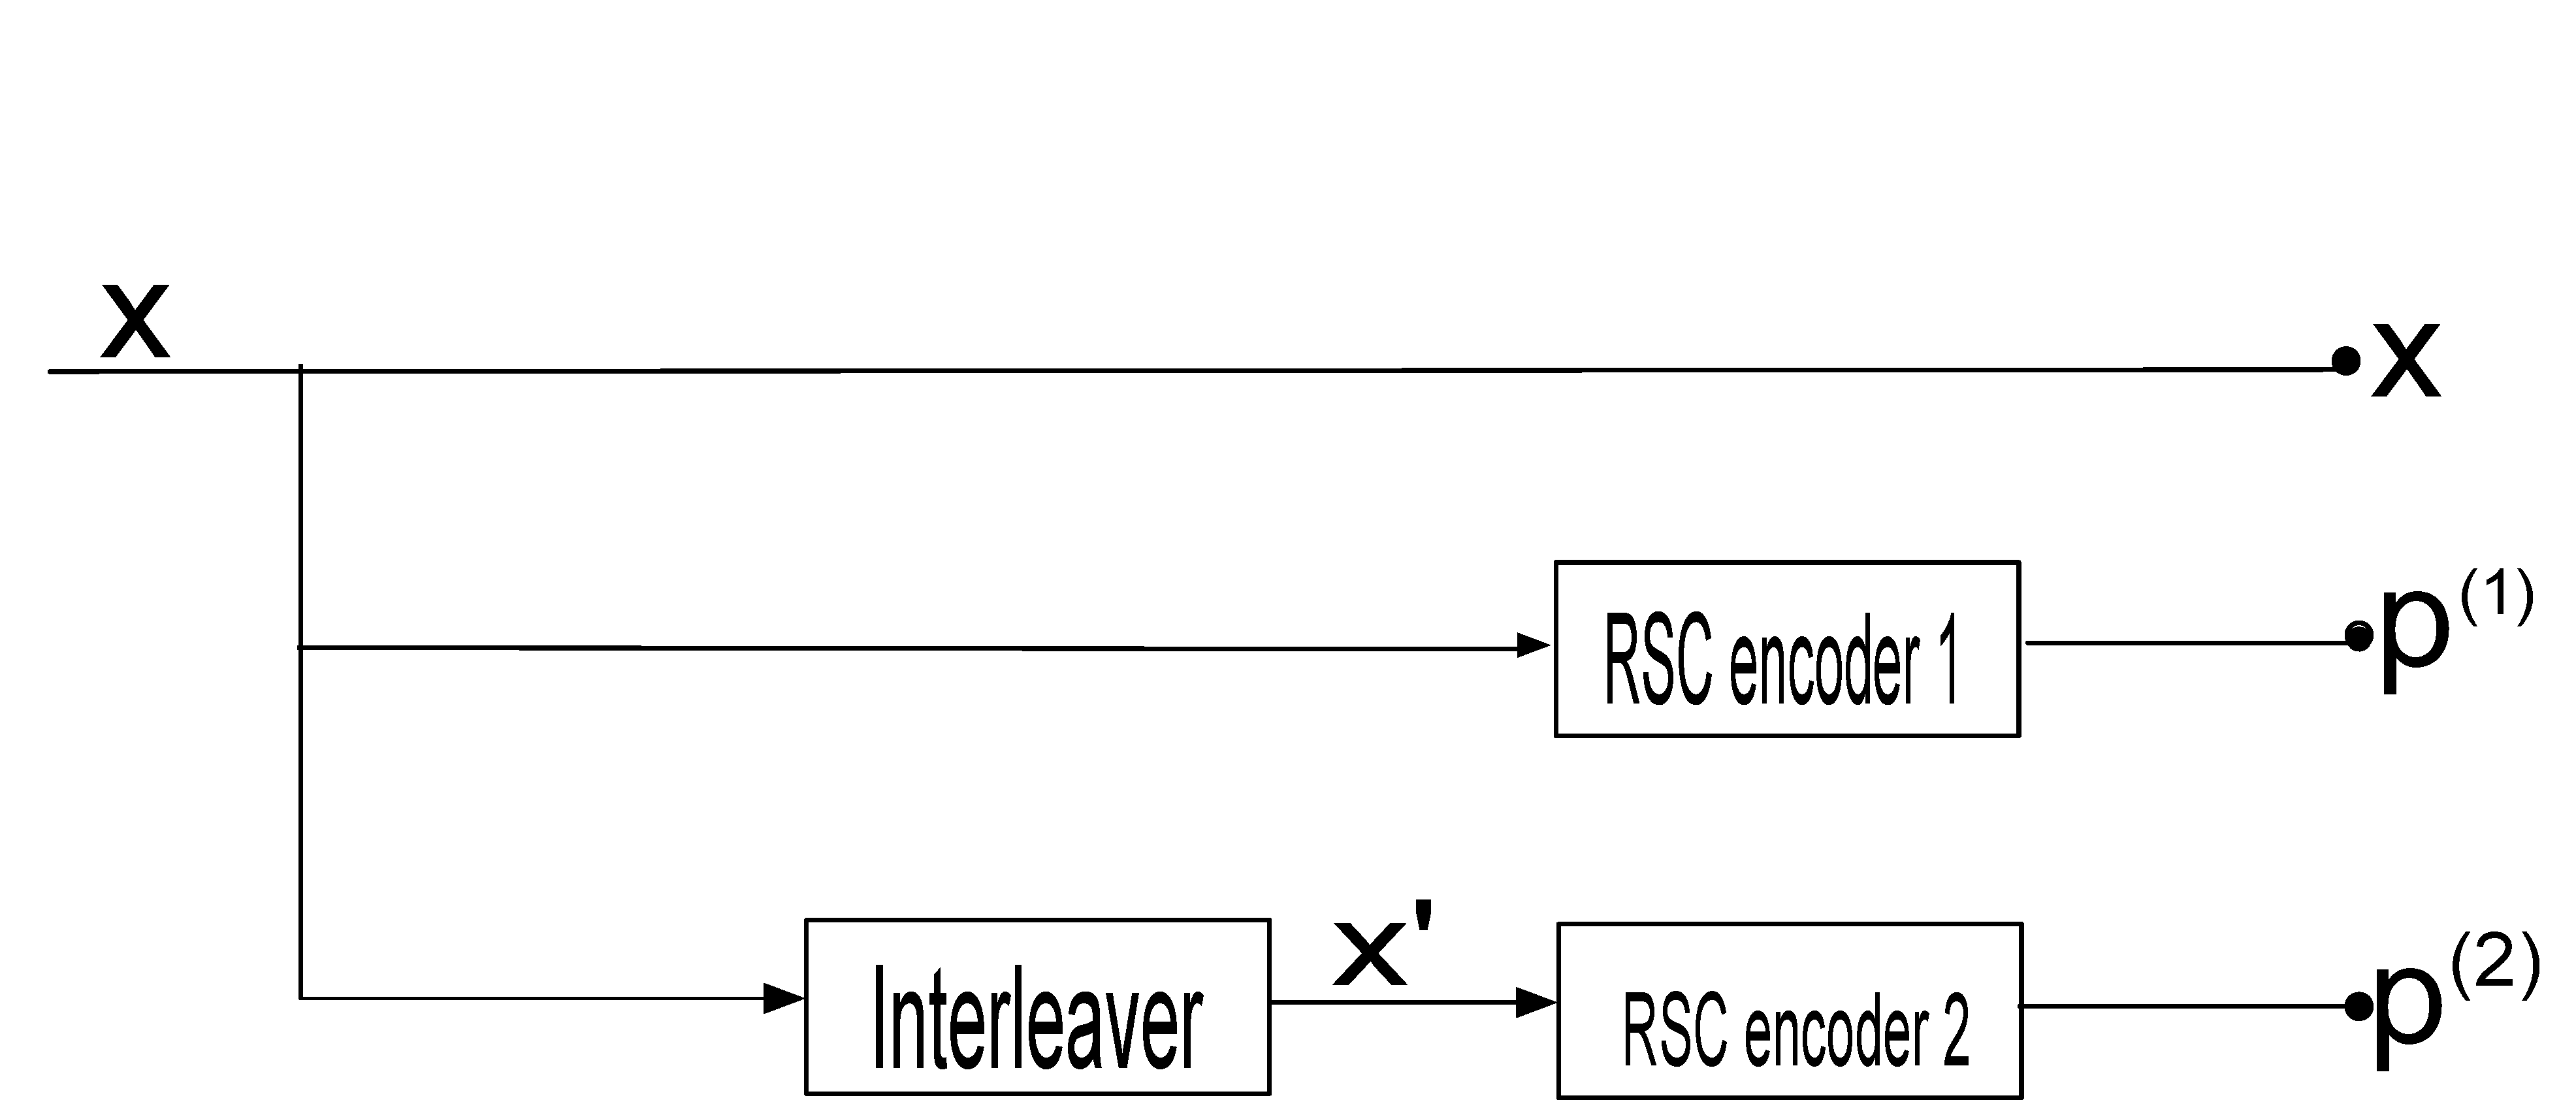
\includegraphics[width = \textwidth]{TurboEncoder.eps}
		\caption{Turbo Encoder}
		\label{TC}
		\end{figure}
	
The system diagram for the turbo encoder is shown in figure(\ref{TC}).
 It is made up of identical Recursive Systematic Convolutional (RSC) encoders which 
 are connected
  in parallel via an interleaver. The RSC encoders have constraint length $K$ and output
  $n$ bits for every $k$ bits input at time $t$.
  From here onward we refer to the RSC encoders as component 
encoders (CE). The generator matrix of the component codes are written in 
the form $[1\,\, \frac{F(D)}{H(D)}]$ or simply as $[\frac{F(D)}{H(D)}]$
where the numerator and the denomenator represent the feedfoward and feedback
 connections of the component encoder. The $''1''$ represents the information 
 (systematic) bits fed into the encoder.

 The generator matrix for the one shown in Figure \ref{RSC}
 is $[\frac{1+D^2}{1+D+D^2}]$ .The encoding process is as follows.

\begin{figure}[h!]
\centering
		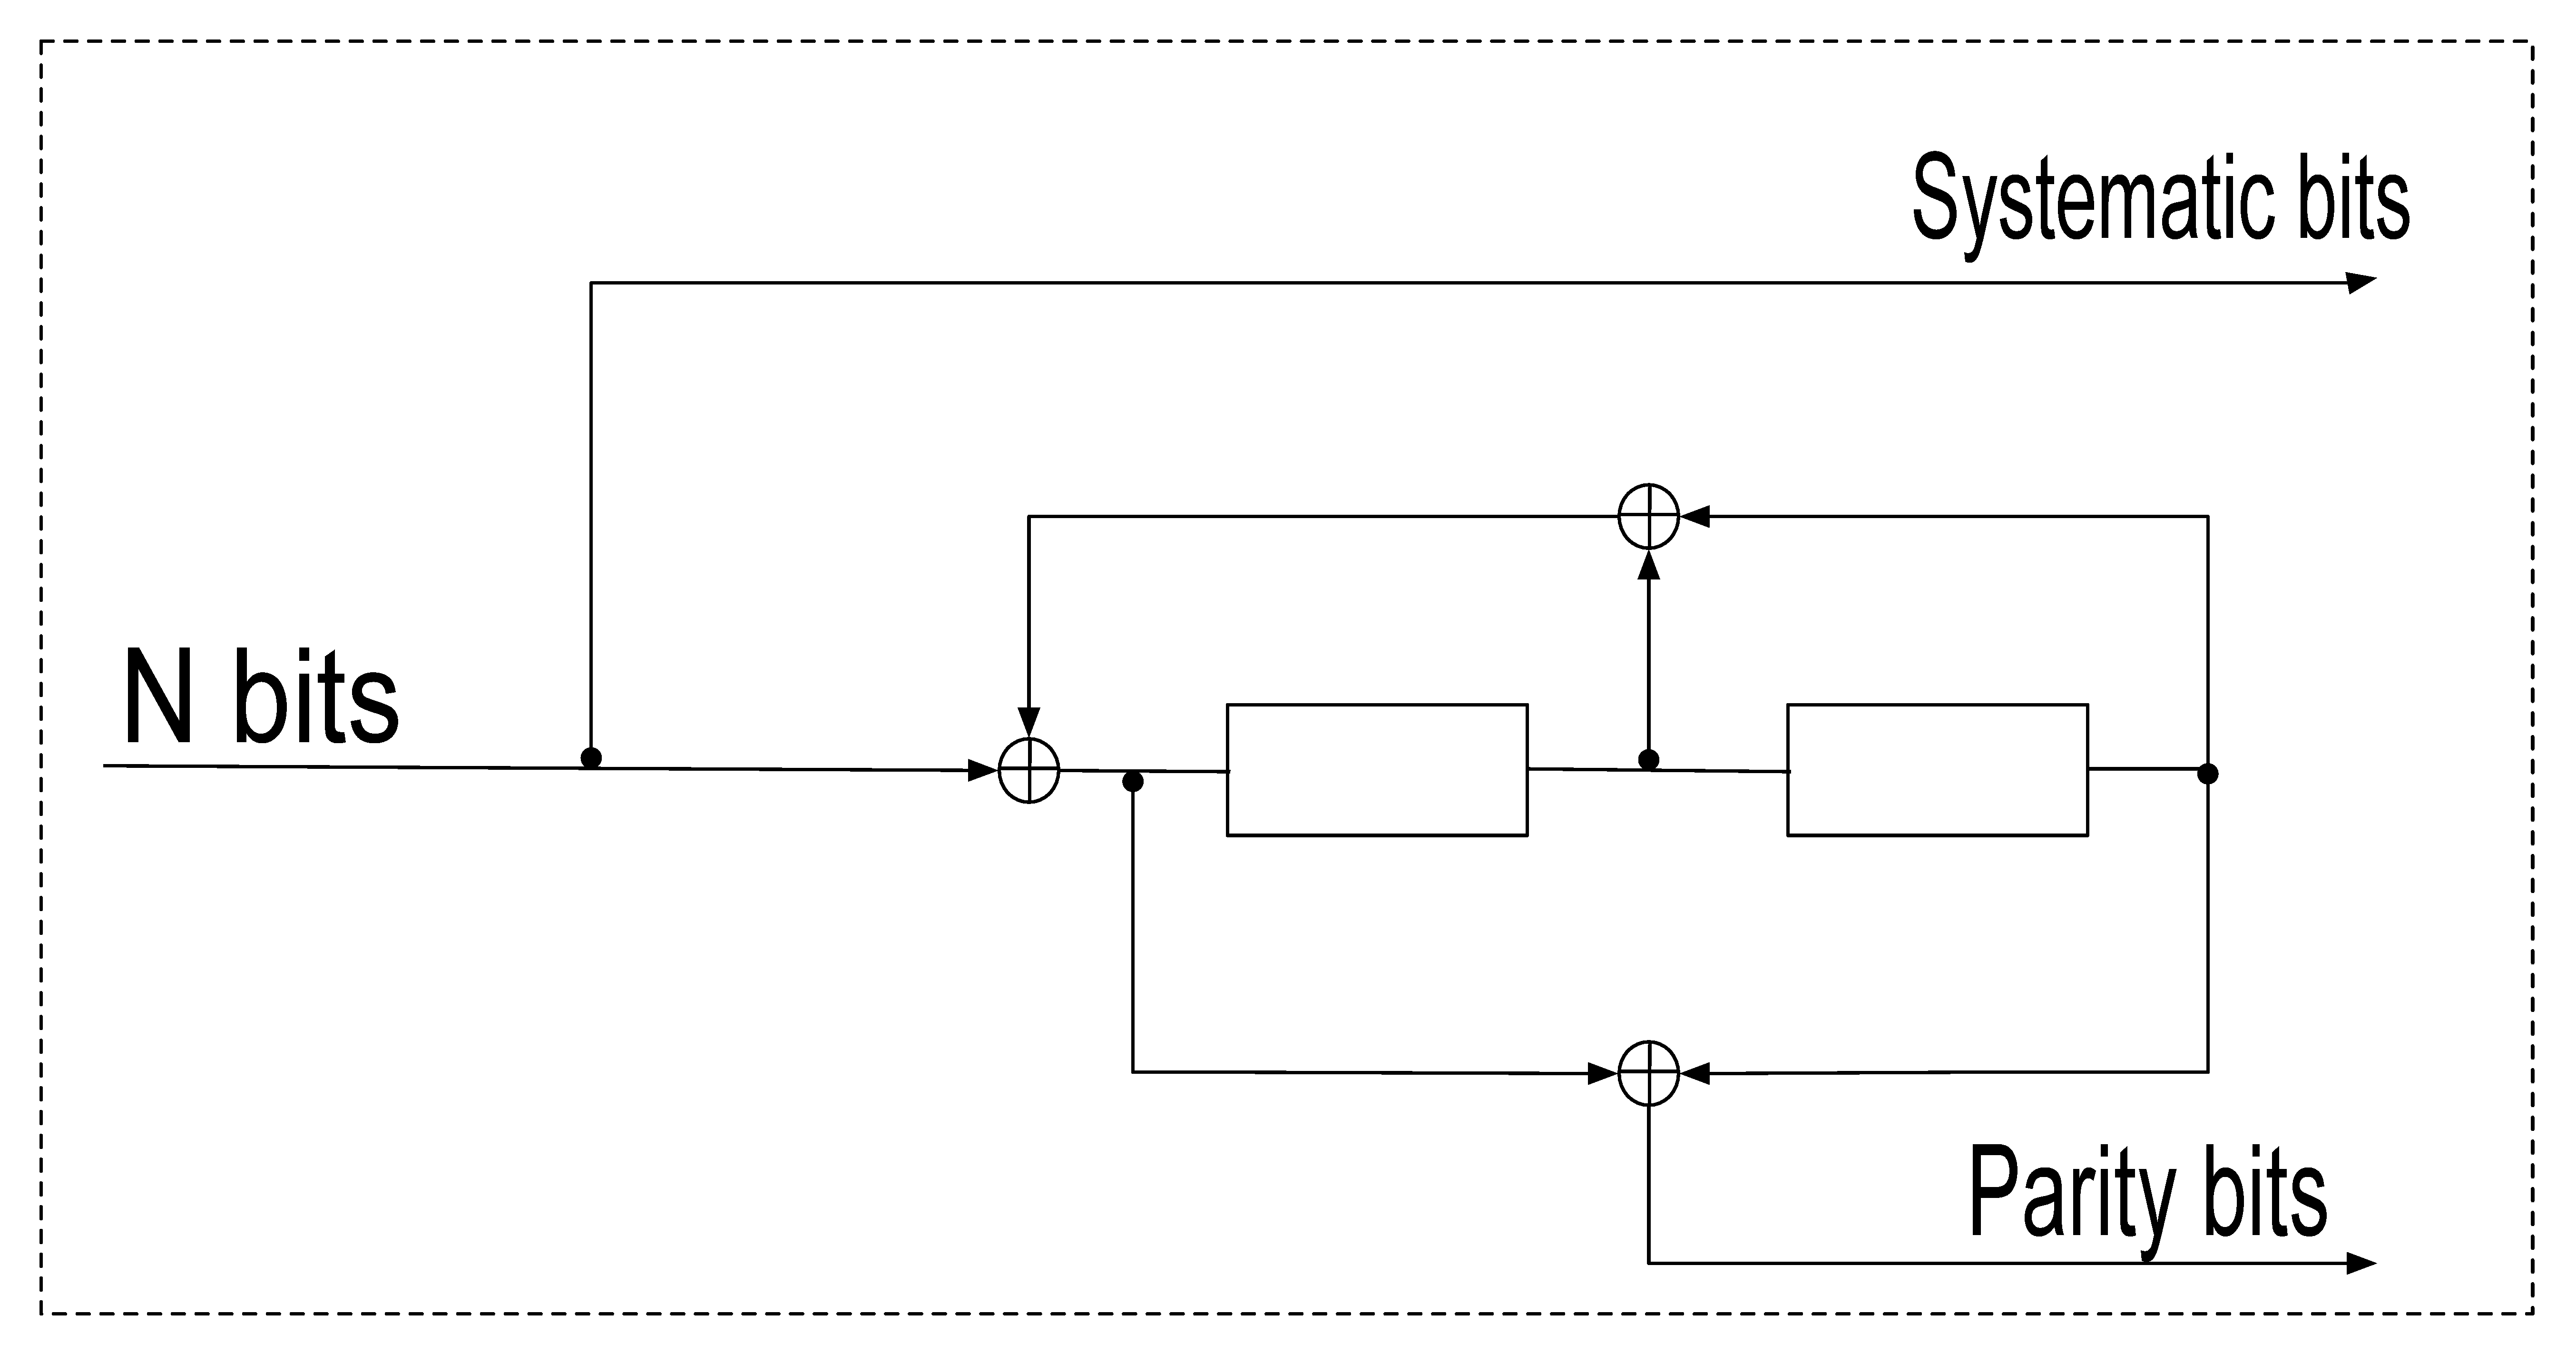
\includegraphics[width=\textwidth]{RSCExample3.eps}
		\caption{$[\frac{1+D^2}{1+D+D^2}]$  RSC Encoder}
		\label{RSC}
		\end{figure}


In our encoding scheme, we terminate the CE1 and leave CE2 open. 
To acheive this,	
 an information sequence $\mathbf{x}=\{x_0,x_1,...,x_{N-M-1} \} $
$M=K-1$
of length $N-m$ is fed into the turbo encoder. This is fed directly into CE1 (assumed to 
begin in the all-zero state) and produces the upper parity sequence 
$\mathbf{p}^{(1)}=\{p^{(1)}_0,p^{(1)}_1,...,p^{(1)}_{N-M-1} \}$ also of 
length $N-M$. 
Since it is desired to return CE1 to the all-zero state, $m$ extras tail bits 
are fed into CE1 which brings the total length of $p^{(1)}$ to $N$. The tail bits are
also added to $\mathbf{x}$ transforming it into a vector of length $N$.
The input to the CE2 (also assumed to 
begin in the all-zero state) is 
$\mathbf{x'}=\Pi(\mathbf{x})= \{x'_0,x'_1,...,x'_{N-1} \} $. This produce the lower 
parity sequence 
$\mathbf{p}^{(2)}=\{p^{(2)}_0,p^{(2)}_1,...,p^{(2)}_{N-1},...,p^{(2)}_{N-1} \}$
 which has total length $N$ since we wish to keep the trellis of CE2 open.
 $\mathbf{x}$ (along with the extra m tail-bits), $\mathbf{p}^{(1)}$
 and $\mathbf{p}^{(2)}$ are multiplexed, BPSK modulated and transmitted over the
 AWGN channel.
 The turbo codeword generated  
 $$\mathbf{c}=\{x_0,p^{(1)}_0,p^{(2)}_0,...,x_{N-1},p^{(1)}_{N-1},p^{(2)}_{N-1} \} $$ 
 has length $3N$ and the
 turbo encoder has rate $R_c=\frac{N-M}{3N}  $
\section{Turbo Decoding}
 The turbo code transmitted over the AWGN channel is received by the turbo decoder as
  $\mathbf{y}=\{\mathbf{y}^x,\mathbf{y}^{p^{(1)}},\mathbf{y}^{p^{(2)}}\}$ 
  of length $3N$, where $\mathbf{y}^x,\mathbf{y}^{p^{(1)}},\mathbf{y}^{p^{(2)}}$
    correspond to the systematic, upper and lower parity sequence respectively.
    $$\mathbf{y}^x=\{y^x_0, y^x_1,...,y^x_{N-1}\}$$ 
    $$\mathbf{y}^{p^{(1)}}=\{y^{p^{(1)}}_0, y^{p^{(1)}}_1,...,y^{p^{(1)}}_{N-1} \}$$
 $$\mathbf{y}^{p^{(2)}}=\{y^{p^{(2)}}_0, y^{p^{(2)}}_1,...,y^{p^{(2)}}_{N-1}\}$$
\begin{figure}[h!]
\centering
		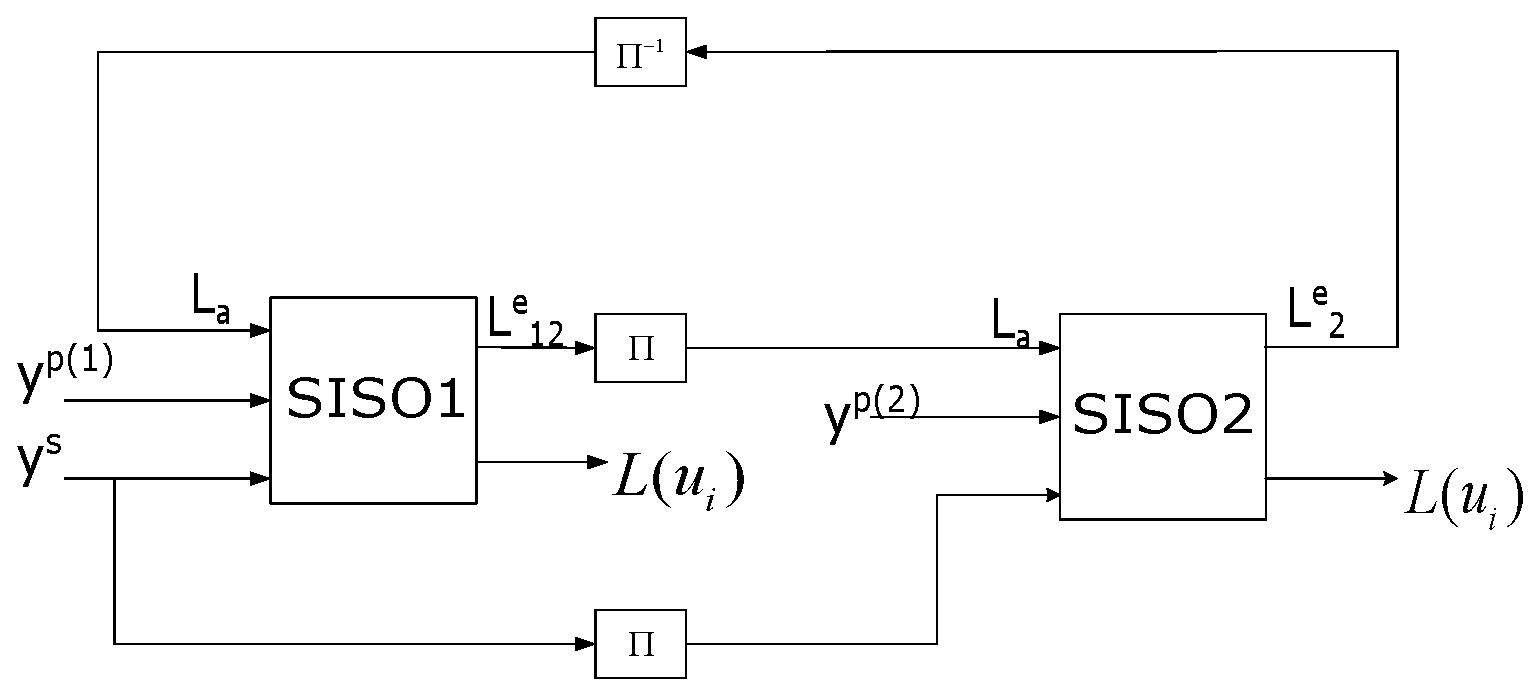
\includegraphics[width=\textwidth]{D1.eps}
		\caption{Turbo Decoder}
		\label{TDC}
		\end{figure}
	
 
 The system diagram for the turbo decoder is shown in figure (\ref{TDC}). It is made up of 2
 Soft Input Soft Output (SISO) decoders (one for each encoder). The decoding 
 process is carried out using turbo decoding algorithm which is based of the use of
 the BCJR algorithm or its variation.  The Max-Log-MAP algorithm is used 
 for its improved numerical stability and simplification of the calculations involved. 
 The algorithm is used to calculate the a posteriori Log-Likelihood Ratio (LLR),  
 $L(x_i|\mathbf{y})=\ln \frac{P(x_i=1|\mathbf{y})}{P(x_i=0|\mathbf{y})}$ 
 of the bits received. This also requires
 the calculation of state transition, feedfoward and feedback probabilities which we
 represent by the symbols $\gamma,\alpha, \beta $ respectively[from BCJR]. We 
 represent the previous trellis state and current trellis state by $\sigma'$ and $\sigma$ 
 respectively.
\begin{equation}
\begin{split}
&\gamma_i(\sigma',\sigma)=
\frac{x_i L_a (x_i)}{2}+
\frac{L_c}{2}\sum_{l=1}^{n} c_{i,l}y_{i,l}\,\,\,\,\, ,\\&L_a(x_i) =\frac{P(x_i=1)}{P(x_i=0)}
\,\,\,\,\, ,Lc=4R_c\frac{E_b}{N_0}\\
&\alpha_i(\sigma)=\max_{\sigma'}[\alpha_{i-1}(\sigma')+\gamma_i(\sigma',\sigma)]\\
&\beta_i(\sigma')=\max_{\sigma}[\beta_{i}(\sigma)+\gamma_i(\sigma',\sigma)]
\end{split}
\label{abc}
\end{equation}
$c_i=\{x_i,p^{v}_i\}\,\,\,\, ,v=1,2$ and the initial values for $\alpha$ and $\beta$ are
\[
    \alpha_0(\sigma)= 
\begin{cases}
   0,& \sigma= 0\\        -\infty,              &  \sigma \neq 0
\end{cases}
\]

\[
   \beta_N(\sigma)= 
\begin{cases}
   0,& \sigma= 0\\        -\infty,              &  \sigma \neq 0
\end{cases}
\]

$ L(x_i)$ is then calculated by using equation (\ref{LLR})
 \begin{equation}
 \begin{split}
 L(x_i)=&\max_{R_1}[\alpha_{i-1}(\sigma')+ \gamma_i(\sigma',\sigma)+\beta_i(\sigma)]
 -\\
 &\max_{R_0}[\alpha_{i-1}(\sigma')+ \gamma_i(\sigma',\sigma)+\beta_i(\sigma)]
\label{LLR}
\end{split}
\end{equation}
where $R_0,R_1$ are the subset of transitions caused by ``0'' and ``1'' respectively.

  The decoding process is as follows.
The input to the SISO1 is $\mathbf{y}^x,\mathbf{y}^{p^{(1)}}$ 
and $\mathbf{L}_a=\{L_a(x_0),L_a(x_1),...,L_a(x_{L})\}$. 
For the first iteration, it is assumed 
that the input information bits have equal probability and $\mathbf{L_a}$ is an 
all-zero vector.
These are used to calculate $\gamma ,\alpha , \beta$ using (\ref{abc})
 and finally
$ L(\mathbf{x})$ using (\ref{LLR}) and $\mathbf{L_e^{(1)}}$ is obtained by subtracting
 $L_c\mathbf{y}^x$  from each element in $ L(\mathbf{x})$ .
$\mathbf{L_e^{(1)}}$ is then
 interleaved and fed into SISO2 as the value for
 $\mathbf{L_a}$ along with an interleaved version of $\mathbf{y}^{x}$ and 
 $ \mathbf{y}^{p^{(2)}}$ which correspond to
 the interleaved systematic bits and the lower parity bits. These are used to calculate 
 $\gamma,\alpha , 
\beta, L(\mathbf{x})$
 and finally the extrinsic LLR values 
of the second component decoder, $\mathbf{L_e^{(2)}}$.
$\mathbf{L_e^{(2)}}$is deinterleaved、and fedback into the first component encoder
 as the new $\mathbf{L_a}$ value for SISO1.

The process is either repeated for a predetermined number of times, or untill a certain 
condition is met. At the final iteration $ L(\mathbf{x})$ (from the second component
 decoder) is deinterleaved and used to estimate the values of $\mathbf{x}$.
 
  It should be noted that, since CE2 was left open, 
 the final state at time $N-1$ could end up being any of the $2^m$ states with 
 probability $\frac{1}{2^m}$. Therefore in SISO2, the initial
 value of $\beta$, $\beta_L(\sigma)=-ln(2^m)$.
 
 \section{RSC encoders and $\tau$-seperated weight error events}
RSC encoders are the component code of choice for turbo codes. They are
characterized by their cycle length ($\tau$) which is defined as the length of the cycle
 of the parity output of the encoder when the input $\mathbf{x}$ is $[1,0,0,0,....]$[5]. 
For example, the RSC encoder in figure (\ref{RSC})has a parity output $\mathbf{y}$ of 
$[1,1,1,0,1,1,0,1,1,0,...]$
for the previously mentioned input. As can be observed, the cycle is $[1,1,0]$ and
the cycle length $\tau=3$. With the knowledge of the cycle and the cycle length $\tau$
of the RSC encoder we wish to explore the effect of weight-$2m$ inputs where the pair of
``1'' bits
 are seperated by $\tau-1$ ` `0' ' bits. We shall refer to to these inputs as
 $\tau$-seperated weight-$2m$ input error events (or simply as $\tau$ weight-$2m$ errors for
 simplicity sake ), where $m={1,2}$. 
In general, the minimum codeword weight associated with weight 2 inputs is known as the effective free distance $(d_{eff})$\cite{ref5}
 Figure(\ref{RSC3})  shows the effect of $\tau$ weight-2 errors on the codeword weight.
 
\begin{figure}[h!]
\centering
		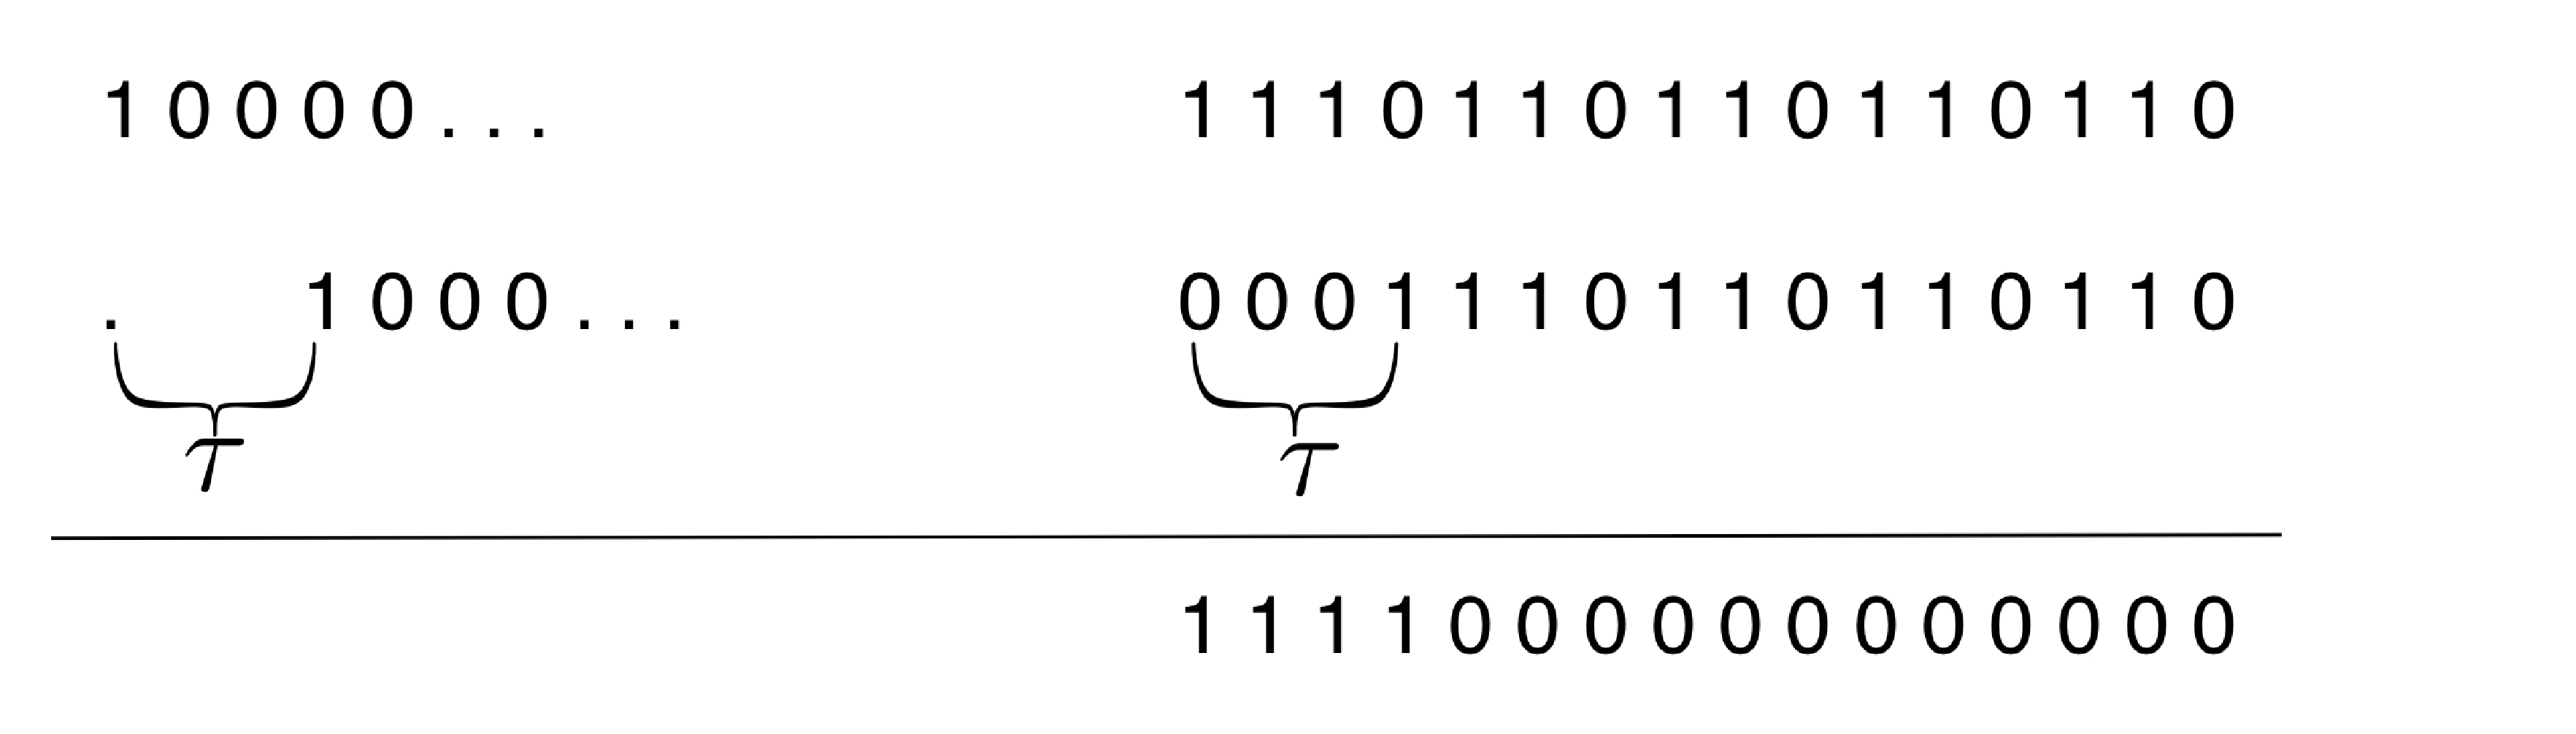
\includegraphics[width=\textwidth]{RSCExample.eps}
		\caption{ effect of $\tau$ weight-2 errors}
		\label{RSC3}
		\end{figure}
	
 The encoder used is the RSC encoder in figure (\ref{RSC})
  and the length $N$ of this vector is assumed to 
be 16. The error vector may then be written as $[1, \mathbf{0}_{\tau-1} 1, \mathbf{0}_{N-\tau+1}]$
(where $\mathbf{0}_z$ is a zero vector of length $z$ ).
This is equivalent to the modulo 2 addition of $\mathbf{x}$ and a version of
 $\mathbf{x}$ shifted by $\tau$ ,$\mathbf{x}_{\Delta\tau}$. As can be seen from 
figure(\ref{RSC3}) these inputs produce parity outputs $\mathbf{y}$ and $\mathbf{y}_{\Delta \tau}$
(version of $\mathbf{y}$ shifted by $\tau$). Modulo 2 addition of $\mathbf{y}$ and
$\mathbf{y}_{\tau}$ result in a low-weight parity output, which inturn results
in a low-weight parity codeword. It can easily be shown that a low-weight parity ouput
will be produced by $\tau$ weight-2 errors irrespective of position of the ``1'' bits . 
%In
%the case of $\tau$ weight-4 errors,the error vector may then be written as
 %$[1 ,\mathbf{0}_{\tau-1},1,\mathbf{0}_{u-1},1,\mathbf{0}_{\tau-1}
% ,1,\mathbf{0}_{N-(u+\tau)}]$ , where $u=2$.

 From the above example, we see that $\tau$ weight-$2m$ errors have the potential to
produce low weight codeword with high multiplicity if they are present in both 
component encoders of the turbo encoder. 
A typical $a-\tau$ weight-$2m$ error event in relation to turbo codes is shown in Figure \ref{2m_error}.

\begin{figure}[h!]
\centering
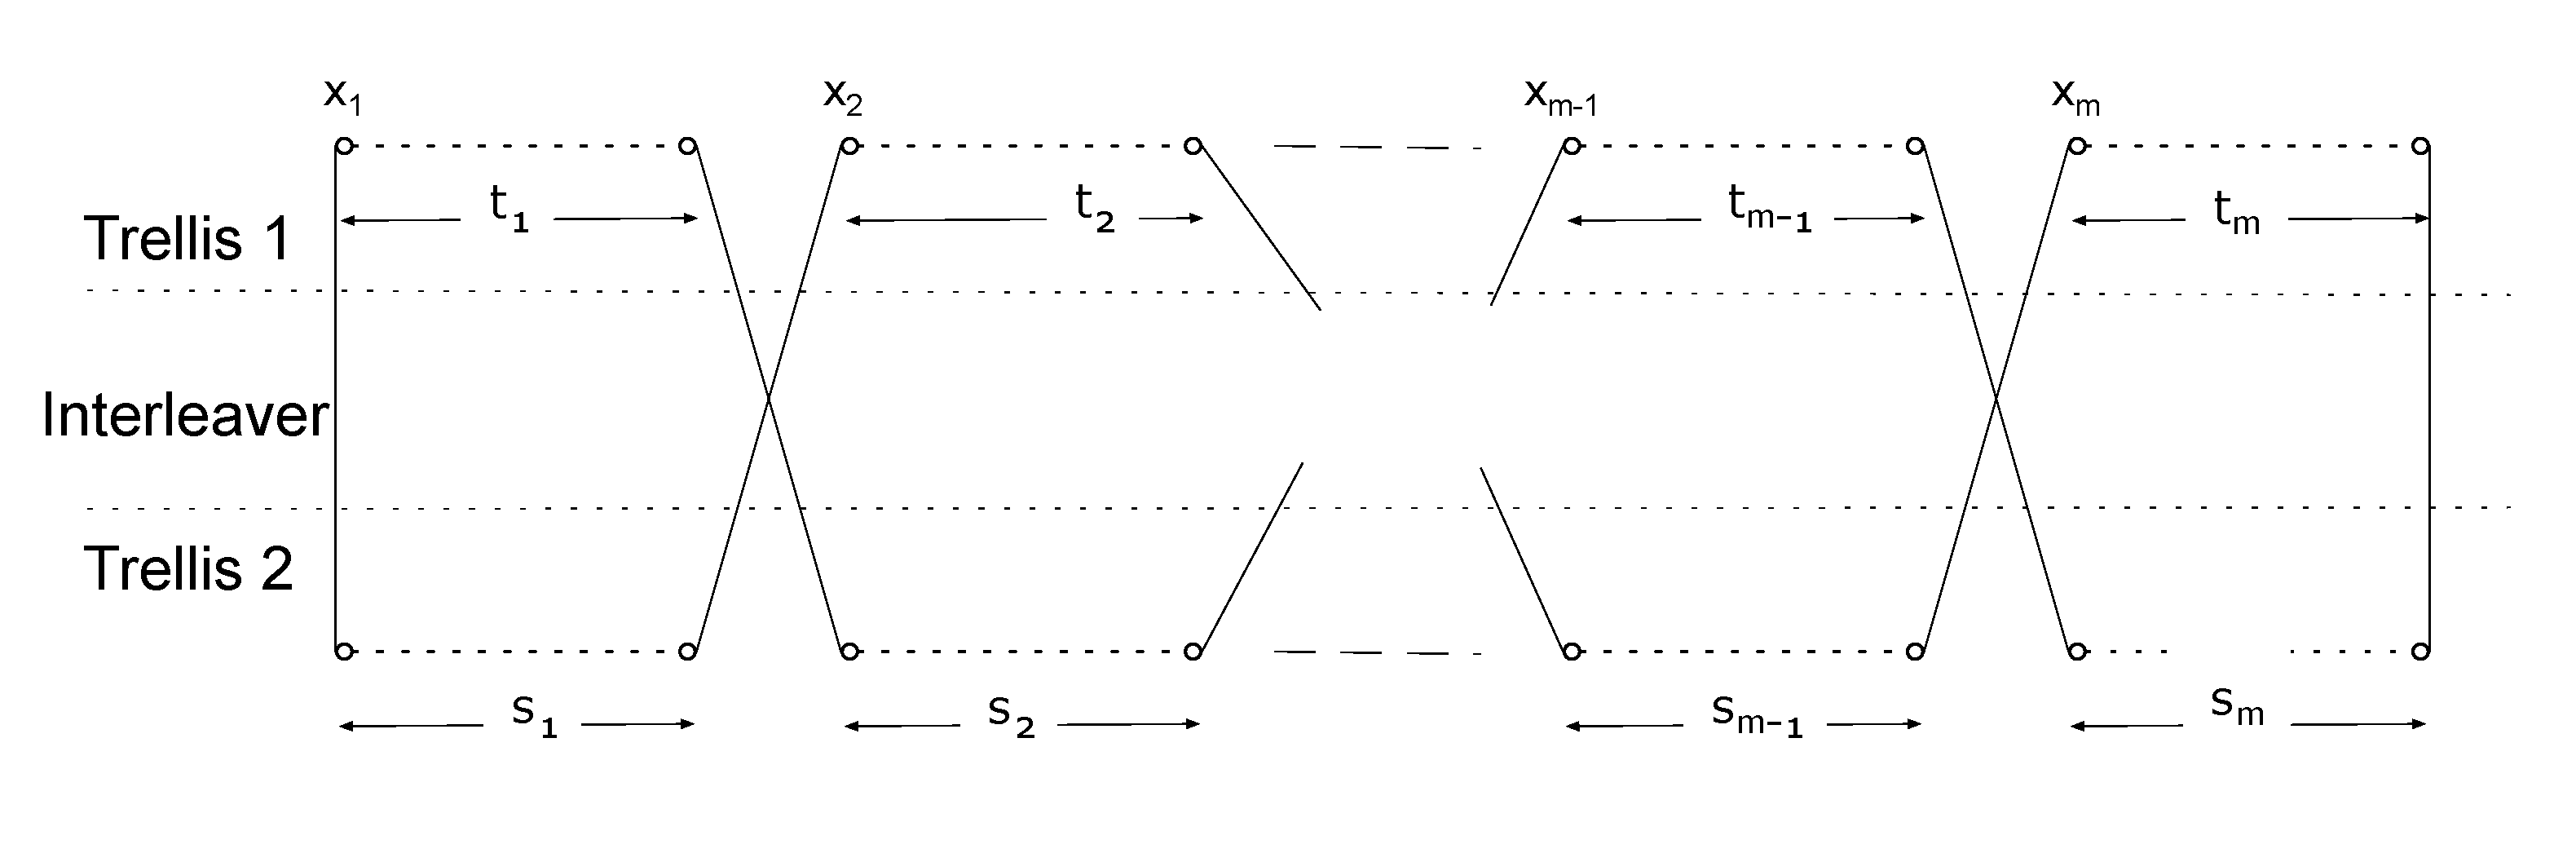
\includegraphics[width=\textwidth]{weight2m.eps}
\caption{$a-\tau$ weight-$2m$ error event}
\label{2m_error}
\end{figure}

 $t_i$ and $s_i$ represent the distance between the $m$ ``1'' bit pairs before and after interleaving repectively. Also, $s$ and $t$ are multiples of $\tau$.

 
\chapter{Interleaver Design for Turbo Codes}
\section{Turbo Codes with Linear Interleavers}

We approach the design of our interleaver by breaking the $a-\tau$ weight-$2m$ error event into smaller subclasses and getting rid of as many errors as possible whiles increasing $d_{eff}$ before moving on to the next subclass. In our analysis we consider 
$a-\tau$ weight-$2m$ errors that originally have a length of $N-M$ and maintain weight $2m$ after $M$ tails bits are added to return CE1 to the all-zero state.

 
 \subsection{Linear Interleaver Design for $a-\tau$ weight-$2$ errors}\label{ss2}
 The linear interleaver is a simple deterministic interleaver based on the circular shifting and its index mapping function is given by
$$ \Pi_{\mathfrak{L}_N}(i) \equiv Di \mod N \,\,\,\,\, 0 \leq i < N, \, gcd(N,D)=1$$
$D$ is reffered to as the interleaver depth. The design of the linear interleaver is essentially picking a suitable value for $D$ for a
given interleaver length $N$ and in \cite{ref2} considerations for choosing a suitable 
value for $D$ is introduced. 

 We begin with
the simplest subclass, which is the $a-\tau$ weight-$2$ error. The error is shown in Figure \ref{2_error} . 
\begin{figure}[h!]
\centering
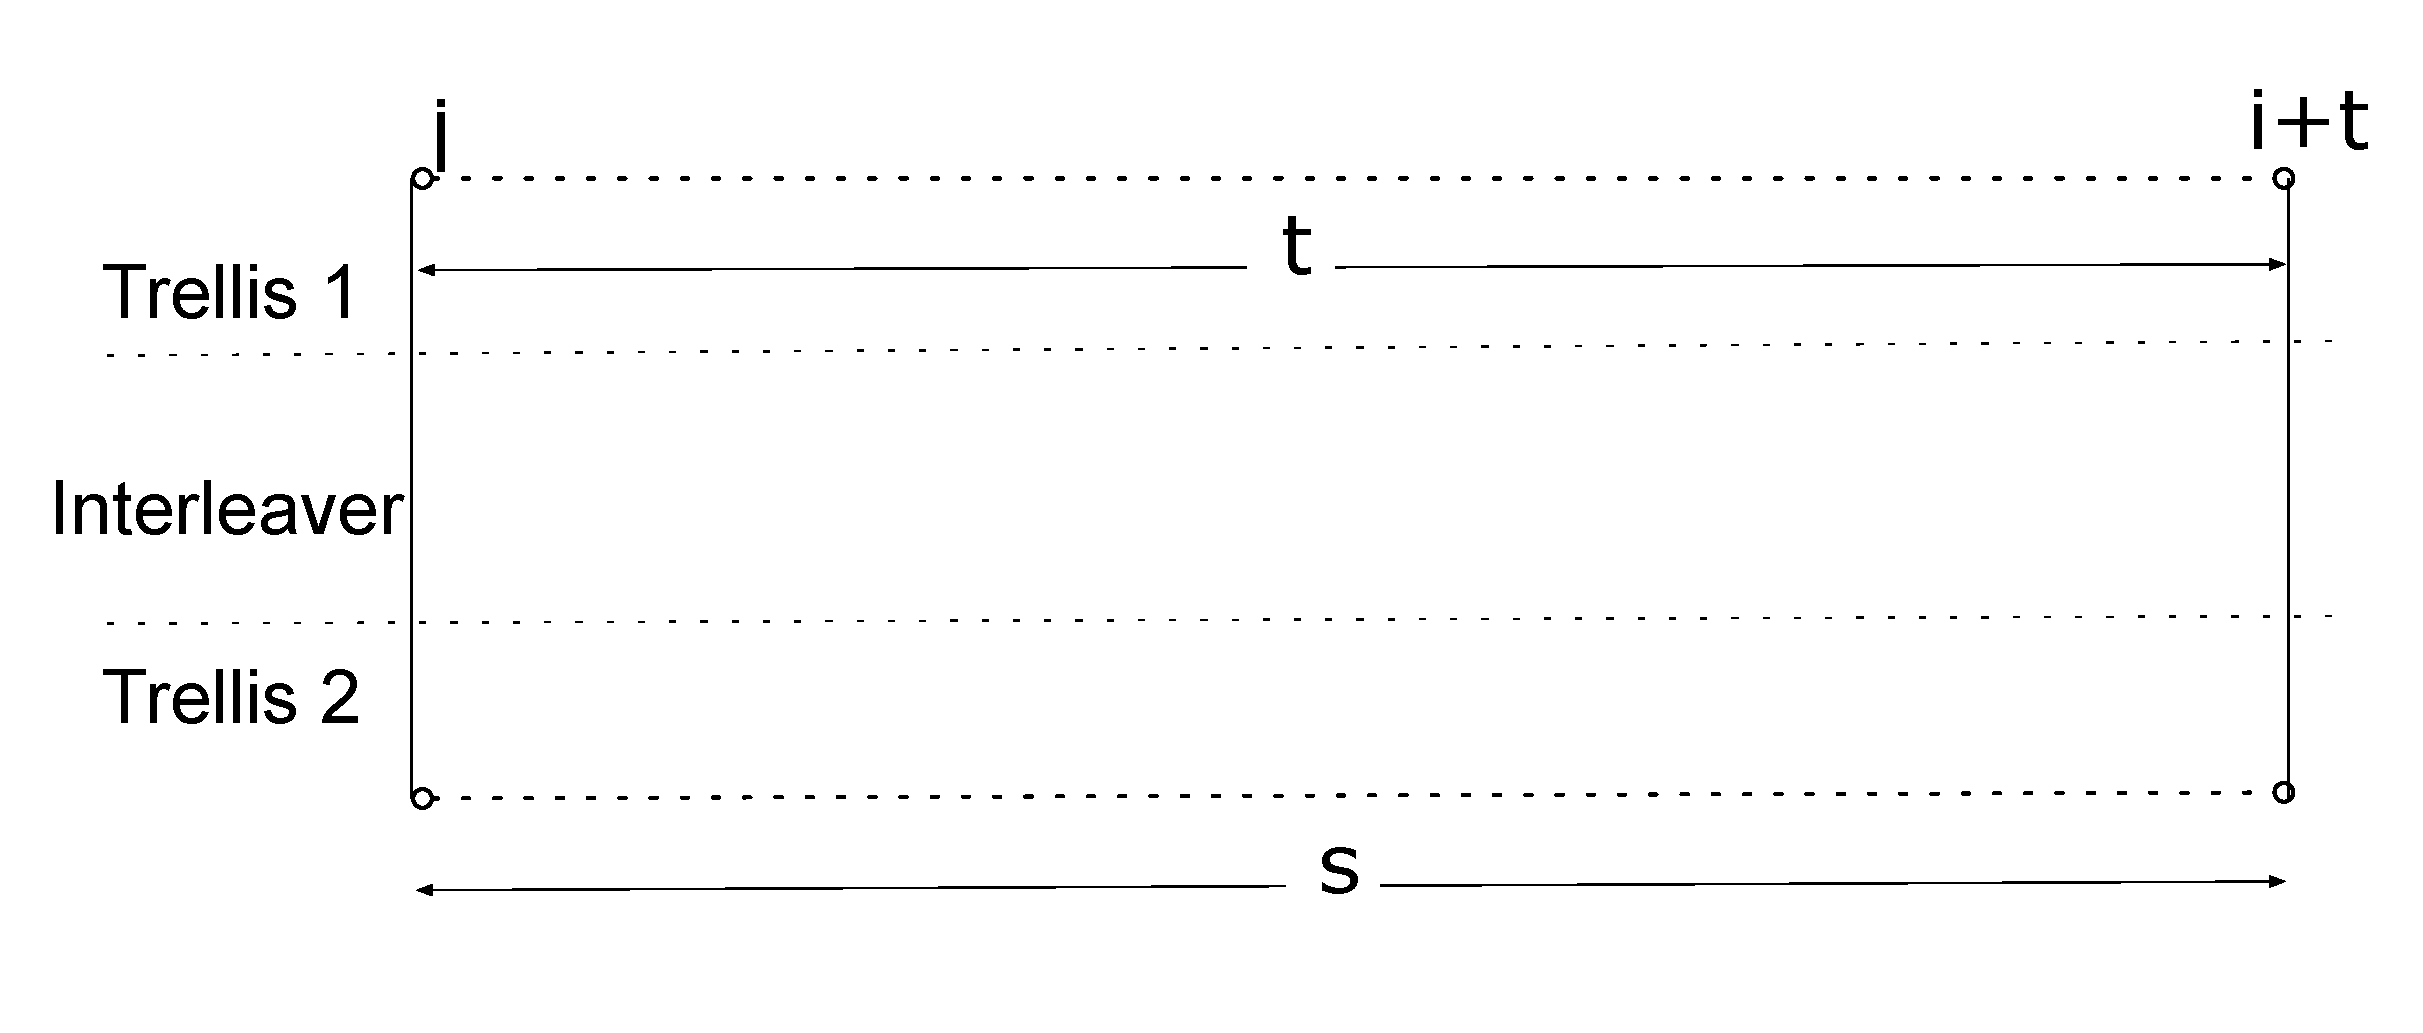
\includegraphics[width=\textwidth]{weight2.eps}
\caption{$a-\tau$ weight-$2$ error event}
\label{2_error}
\end{figure}
We attempt to design linear interleavers to get rid of such errors.
Assuming the error event at the first encoder begins at $i$ and the ``1'' bit pairs are seperated by a distance of $t$, 
\begin{equation}
\begin{split}
s = &D(i+t) - D(i) \mod N\\
&= Dt \mod N
\end{split}
\label{distrel}
\end{equation}


in the case where $t=a\tau$ and $s=b\tau$, a low weight codeword may be produced. To prevent this error event from occuring we choose $D$ that produces the largest value of $\min t+s$. In the case where there are multiple values of $D$ that satisfy the above condition, we calculate the codeweight word associated with $a-\tau$ seperated weight 2 error events of length $N-M$ and choose the value of D that produces the largest value of effective free distance. 
The procedure for choosing the best linear interleaver is shown below.

[1]. For $D \in (3,N/2), \,\,\, gcd(D,N)=1$, calculate $s$ and  $-s$ using (\ref{distrel}) for all values of $t=a\tau$ and  $t=-a\tau$ respectively.

[2]. For all valid pairs, sum all $(t,s)$ pairs and record $\min (a+b)$

[3]. After this process is repeated for all values of $D$, choose the value of $D$ that produces the largest value of $\min (t+s)$

[4]. In the case where more than one value of $ D$ satisfies the condition we calculate the $d_{eff}$ for each value of $D$ and select the value of $D$ with the largest  value of $d_{eff}$

For an interleaver size of $N=2^8$, and the $5/7$ RSC compenent encoder we use the above procedure to find the best value of $D$ which are $D=13$ and $D=121$. The results are shown in Table \ref{tab1}. The corresponding values of $t$, $s$, $d_{eff}$ and the multiplicity $N_{free}$. In the same table we compare the best values of $D$ with other $D$ values close $\sqrt{N}$. We see that the weight produced by $D=13$ and $D=121$ have the largest value of $d_{eff}$ and therefore should bave a better decoding performance.

\begin{table}[h!]
\centering
\begin{tabular}{||c |c |c |c |c |c ||} 
 \hline
 $D$ & 13 & 121 & 17 & 23 & 21\\ [0.5ex] 
 \hline\hline
 $t $ & 21 & 15 & 15 & 12 & 21 \\ 
 \hline
  $s $ & 17 & 23 & 1 & 20 & 4 \\ 
  \hline
  $d_{eff} $ & 30 & 30 & 15 & 26 & 15 \\ 
  \hline
  $N_{free}$ & 1 & 1 & 2 & 1 & 2 \\ [1ex] 
 \hline
\end{tabular}
\caption{Best value of $D$ for $N=256$ linear interleaver
 and $5/7$ component encoder. }
\label{tab1}
\end{table}

The Bit Error Rate (BER) upper bound for Turbo is derived in \cite{ref6} and is given by (\ref{aprox}).

\begin{equation} 
 P_e \approx \frac{1}{2}\sum_{w_c}D_{w_c} 
  erfc \Bigg(\sqrt{w_c\frac{R_cE_b}{N_o}} \Bigg)
  \label{aprox}
  \end{equation}
 where 
  $$ D_{w_c}\triangleq \sum_{w_x+w_p=w_c} \frac{w_x}{N}A_{w_x,w_p}$$
  $w_x$ is the weight of the input sequence, $w_p$ is the weight of the parity 
  sequence,$R_c$ is the rate of the turbo code , $w_c$ is the weight of the turbo 
  codeword and $A_{w_x,w_p}$ is the multiplicity of $w_c$. Using  (\ref{aprox}), we estimate the BER performance of the turbo codes constructed using linear interleavers. From Table \ref{tab1} we plot the BER curve for $D=121$, $D=23$ and $D=21$. We also run simulations for $D=121$ and compare it to its BER curve as shhown in figure \ref{t1comp}. 
  
  \begin{figure}[h!]
\centering
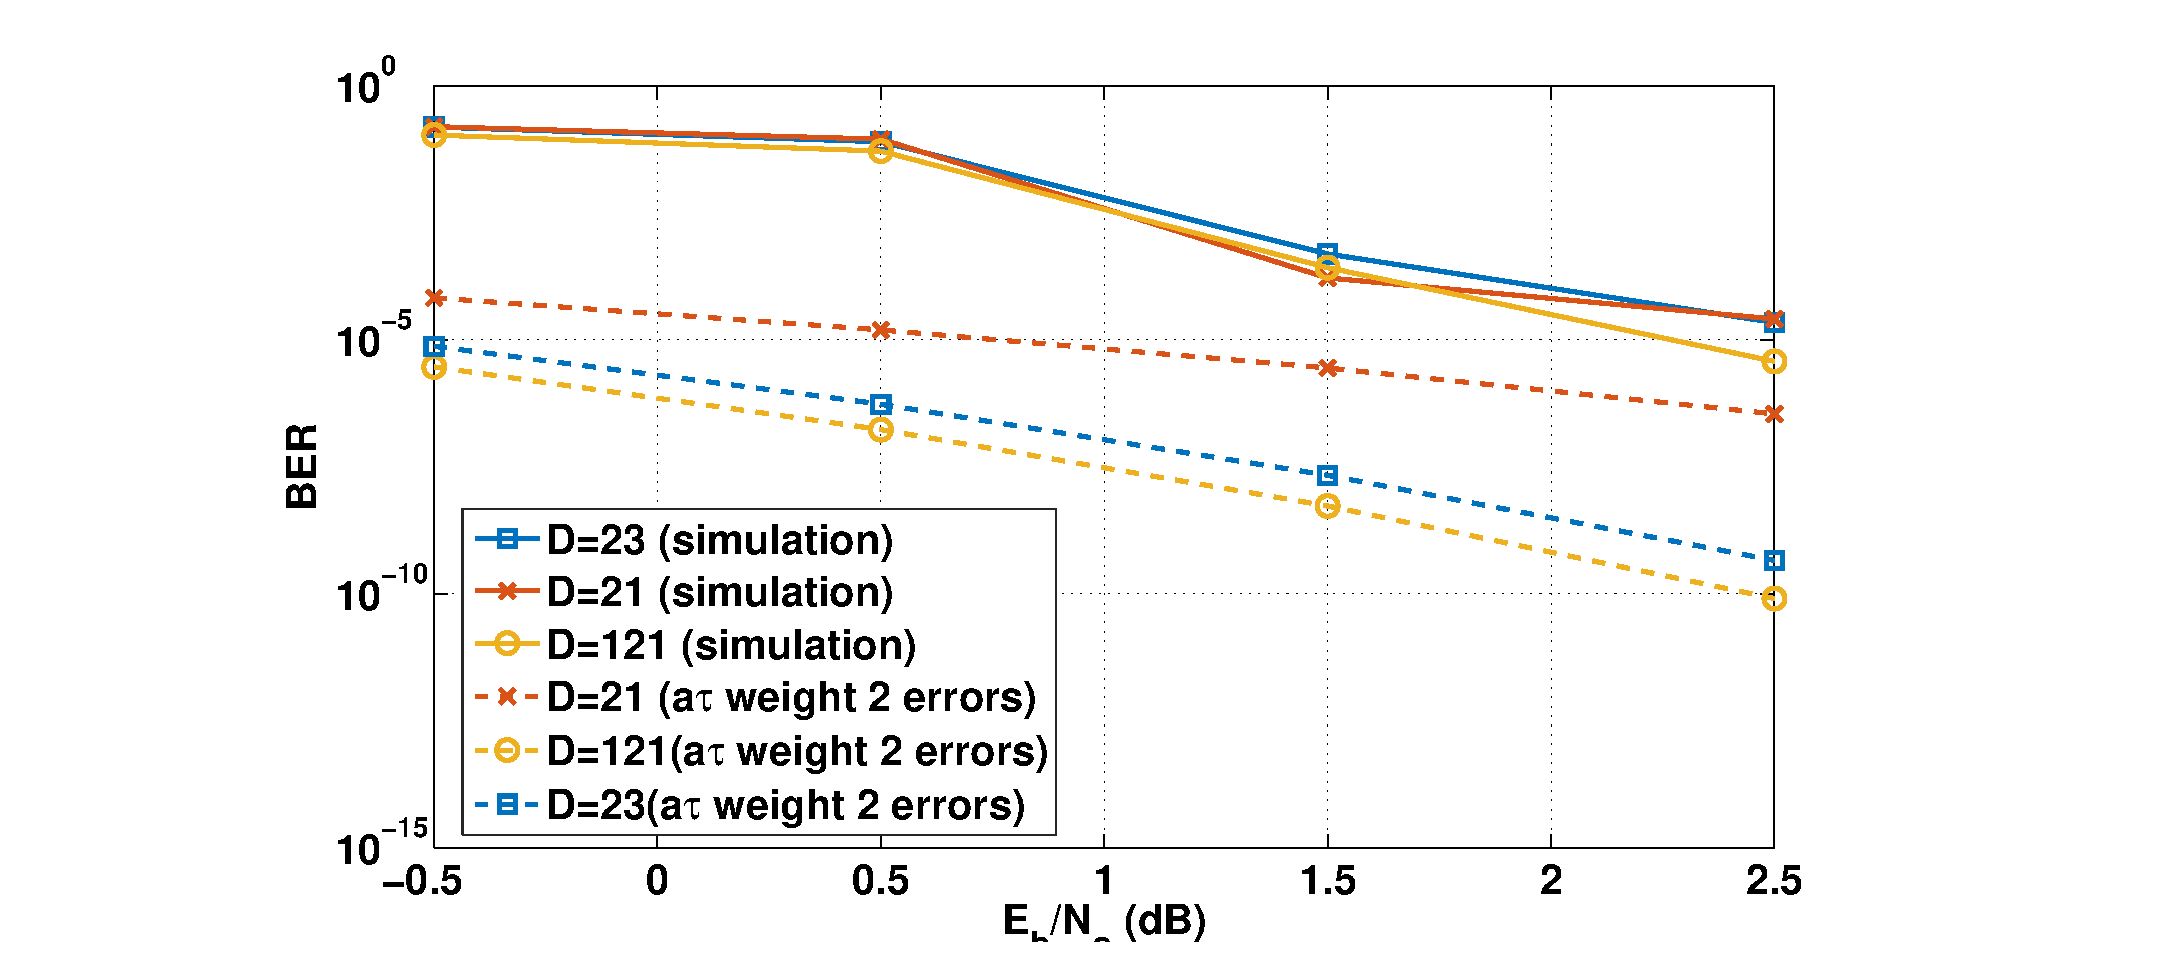
\includegraphics[width=\textwidth]{D_23_21_121_N_256.eps}
\caption{Theoretical and simulation results for $D=21$, $D=23$ and $D=121$}
\label{t1comp}
\end{figure}
  
  We realize that the estimated BER curve fails to properly estimate the simulated BER performance. This suggests that there exists codeword with weight lower $d_{eff}$ caused by higher weight error events. We therefore proceed to the next error subclass which is the $a-\tau$ weight $4$ error subclass.
\subsection{Linear Interleavers and $a-\tau$ weight-$4$ errors}\label{sstau}
%%%%%%%%%%%%%%%%%%%%%%%%%%%%%%%%%%%%%%%%%%
A typical $a-\tau$ weight-$4$ error event is shown in Figure \ref{4_error}. It is made up of $2$ ``1'' bit pairs with the paired bits seperated by a distances of $t_1$ and $t_2$ respectively. After interleaving the distances are mapped to $s_1$ and $s_2$ respectively. 
\begin{figure}[h!]
\centering
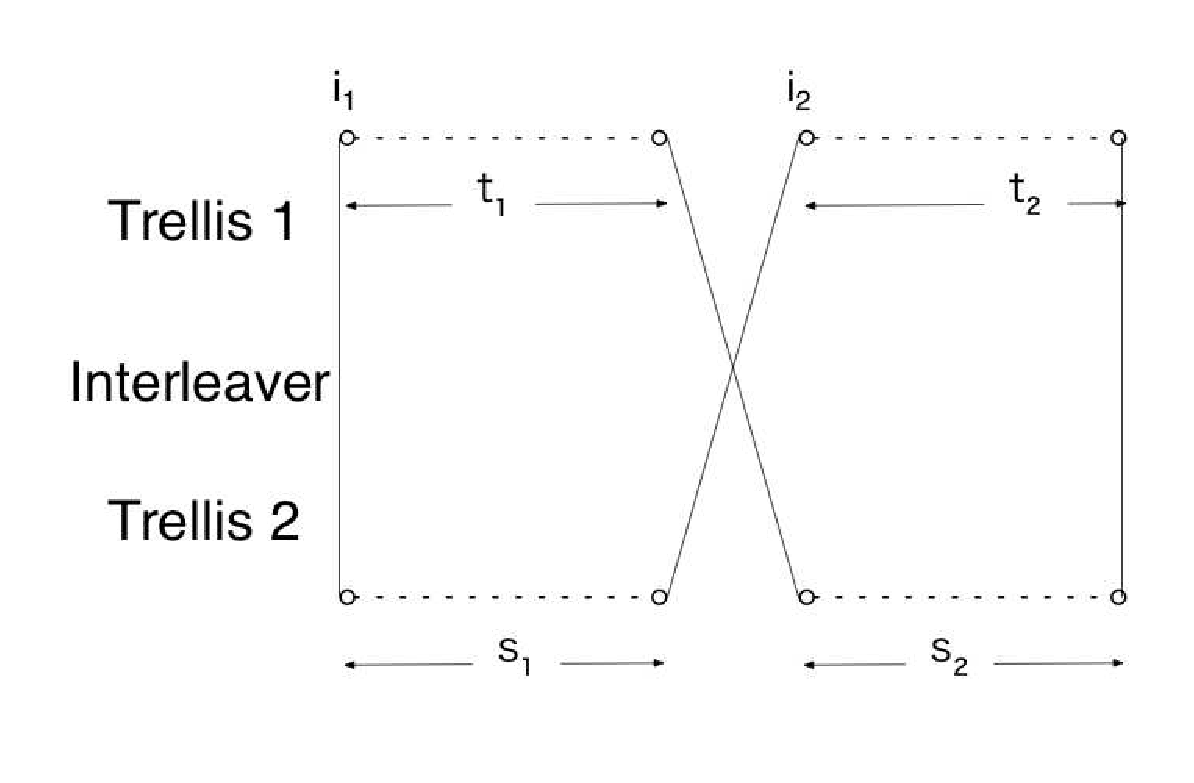
\includegraphics[width=0.8\textwidth]{weight4.eps}
\caption{$a-\tau$ weight-$4$ error event}
\label{4_error}
\end{figure}
We begin with the case where $t_1 = t_2 =\tau$. 
For linear interleavers, there exists an input distance $t=v$ or $t=w=-v \mod N$ such that the output distance $s=\tau$. The relationship between $D$ and $v$ is a result of the following linear congruence relationship 
\begin{equation}
 Dv \equiv \tau \mod N
 \label{lincong}
 \end{equation}
Given the value of $D$ the value of $v$ can easily be solved for. If $t_1$ and $t_2$ are seperated by a distance $ dp= v - \tau$ or  $dp= w - \tau$,  $s_1 = s_2 =\tau$ as shown in
\ref{wt4example}a and \ref{wt4example}b. This output is valid for all $N-(v-\tau)$ times when the position of the ``1'' bits are shifted to the right causing the codeword weight produced to have a high multiplicity. However, there exists cases where $s_1 \neq s_2 \neq \tau$ when  $dp= w - \tau$ as shown in Figure \ref{wt4example}c where the value of $D=121$ and $N = 256$. 

\begin{figure}[h!]
\centering
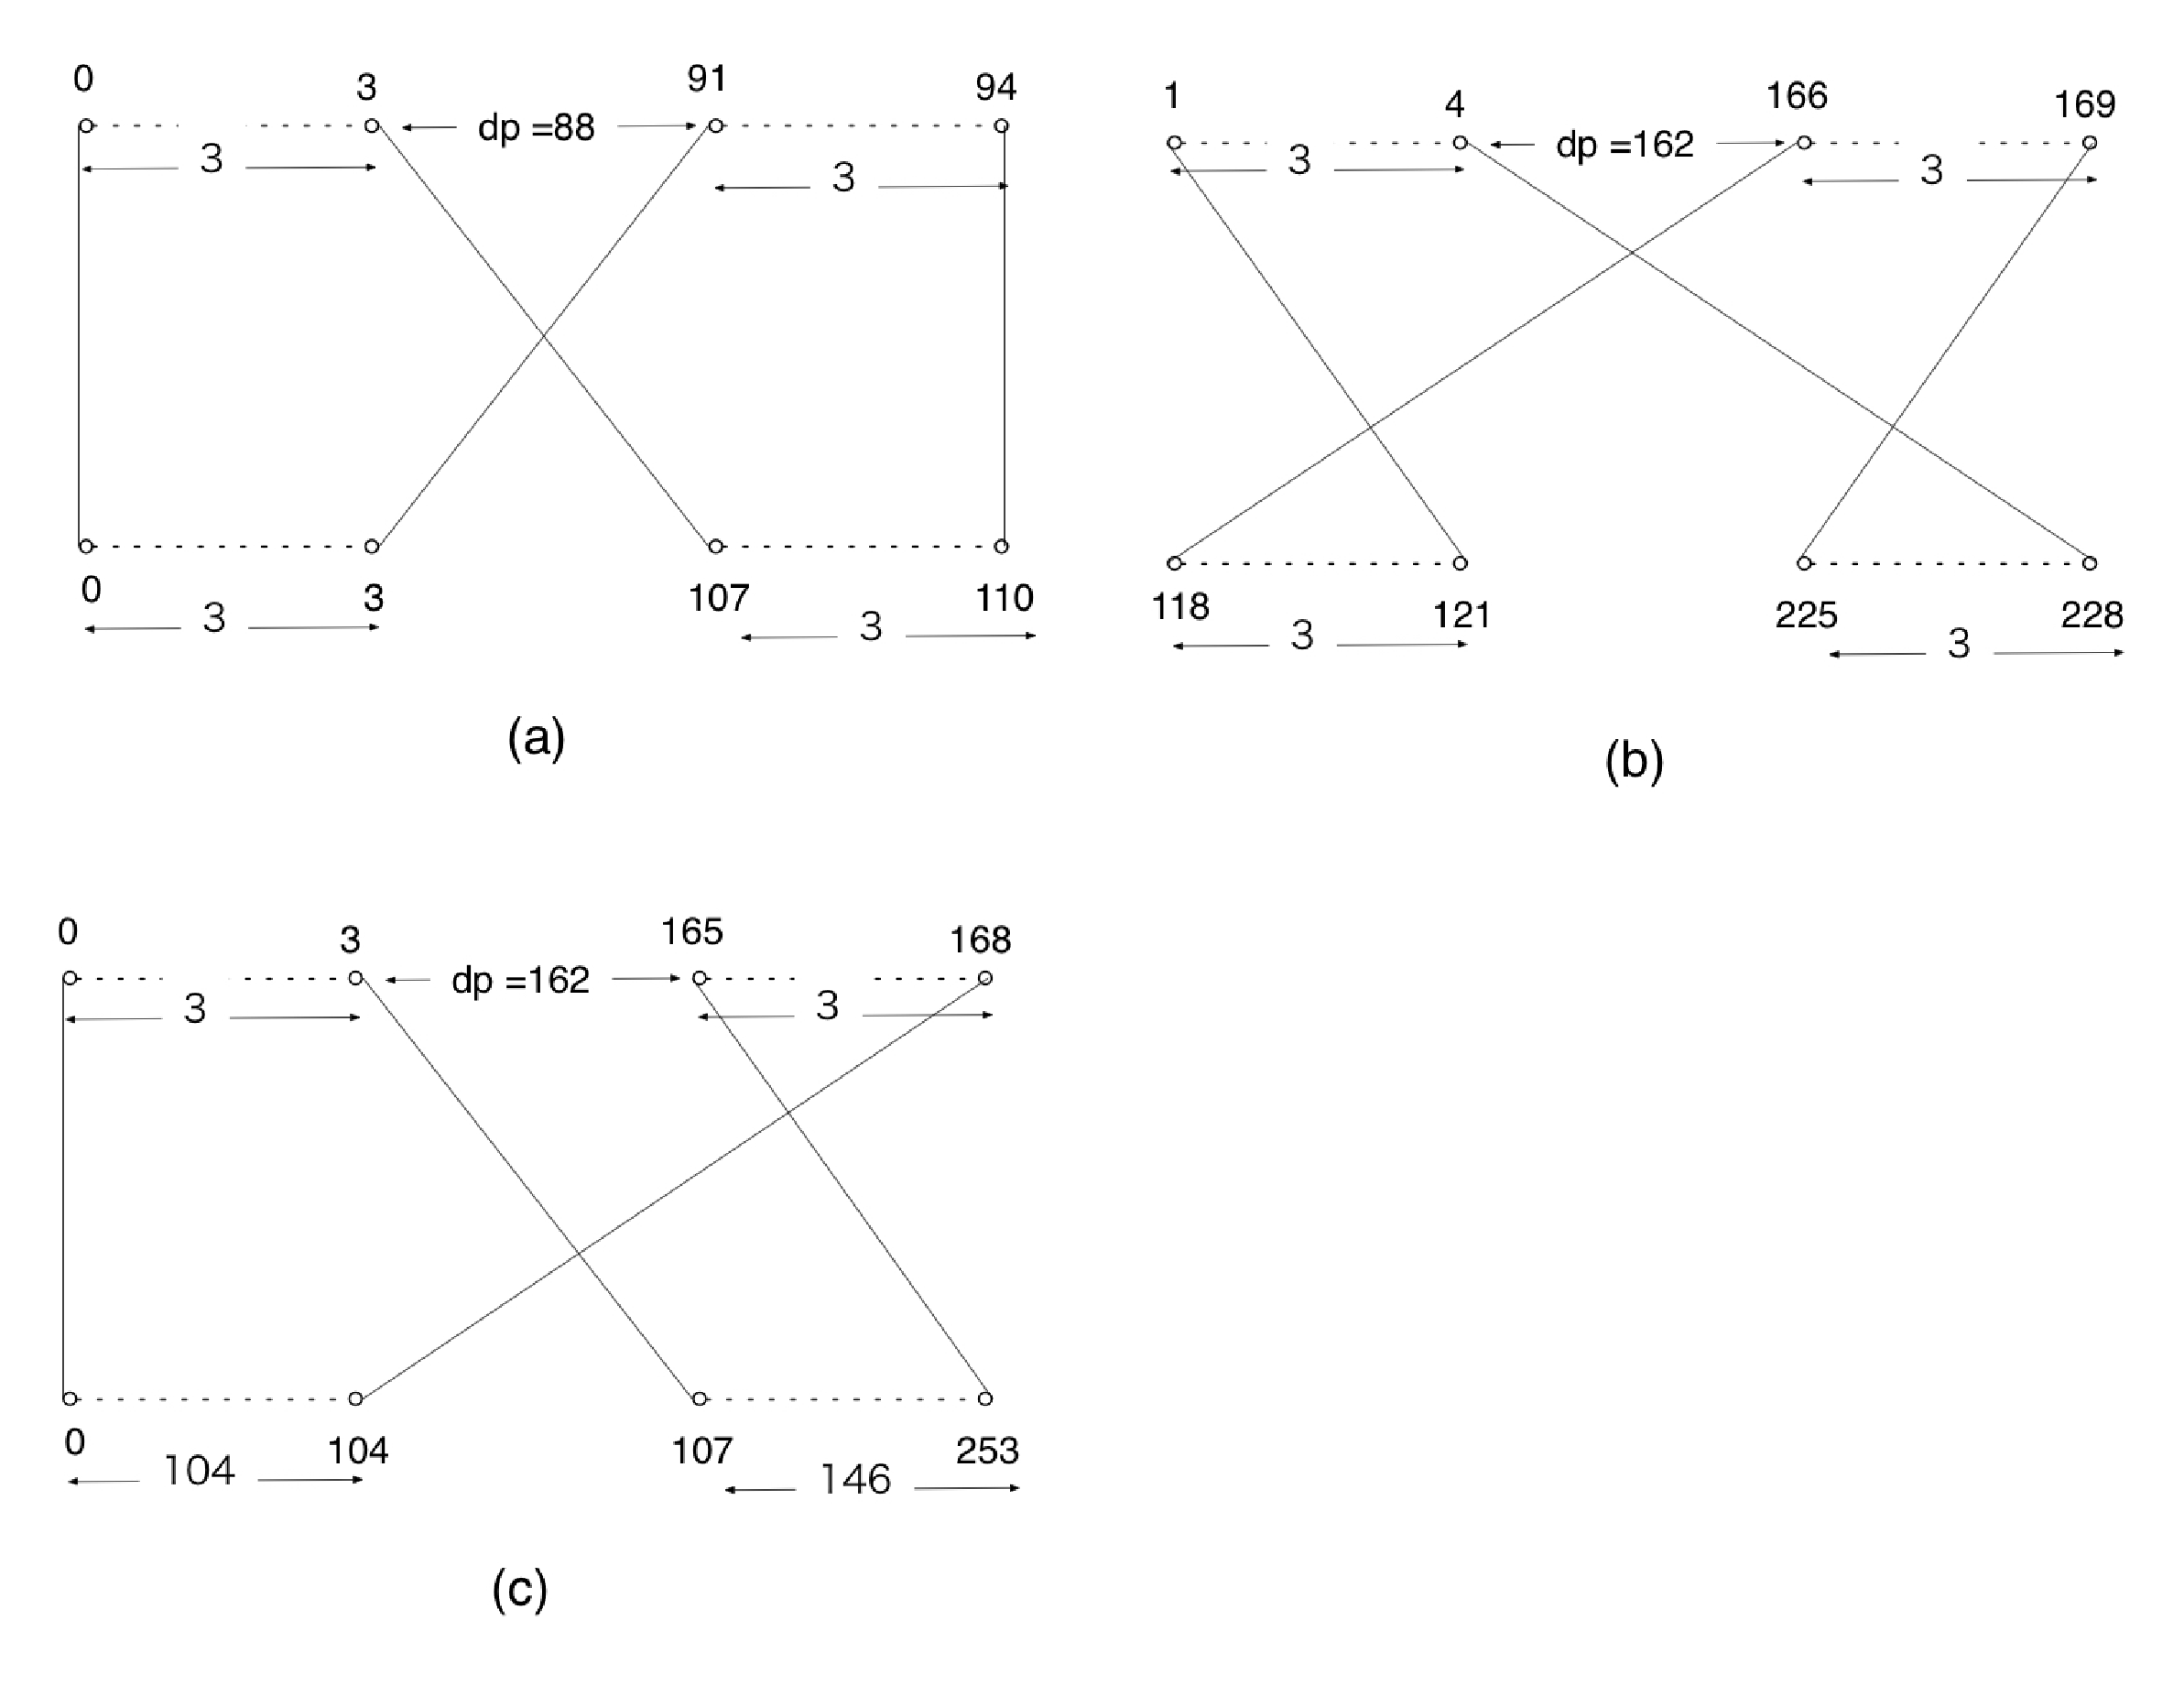
\includegraphics[width=\textwidth]{exampleswt4.eps}
\caption{$a-\tau$ weight-$4$ error event mapping, $D=121$, $N=256$}
\label{wt4example}
\end{figure}

 Also the lowest codeword weight produced has a value of $20$ and due to the large multiplicity, it dominated the BER performance of the turbo. The upper bound BER curve due to $\tau$ - seperated weight $4$ errors is shown in figure \ref{w4bound} and compared to the simulation results obtained when $D= 121$ and $N=256$. It is observed that this curve gives a tighter upper bound on the BER performance of the turbo code.
 \begin{figure}[h!]
\centering
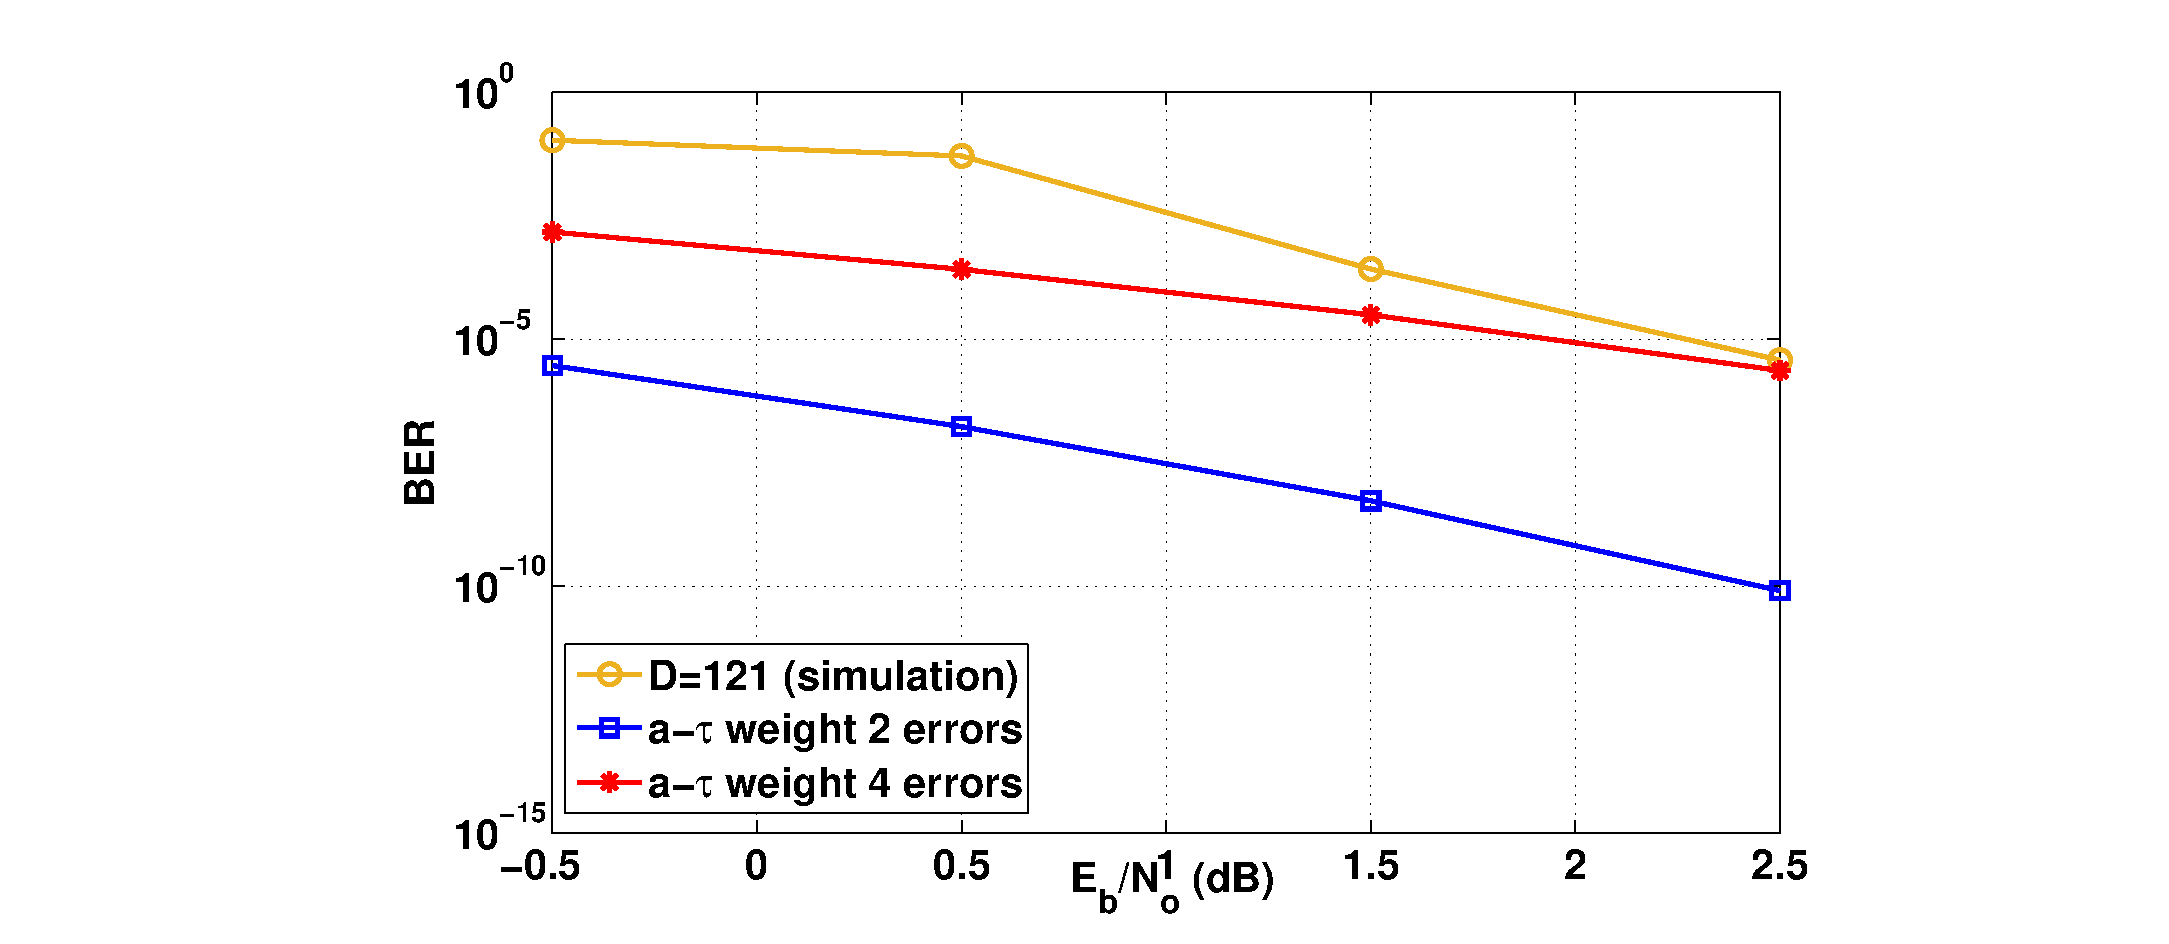
\includegraphics[width=\textwidth]{D_121_N_256_sim_vs_theory.eps}
\caption{Simulation Results vs weight -2 and weight -4 Bounds, $D=121$, $N=256$}
\label{wt4bound}
\end{figure}
 These $\tau$ - seperated weight $4$ errors present a big problem for linear interleaver design. This is because as the value of $N$ is increased it is possible to acheive large values for $d_{eff}$ via the method in Section \ref{ss2}. However the minimum codeword weight resulting from $\tau$ - seperated weight $4$ errors remains constant for a given component code and increases in multiplicity as $N$ increases \cite{ref2}.
 
 \section{Turbo Codes with Multi-Shift Interleaver}
 We propose a method to solve the  $\tau$ - seperated weight $4$ errors dominating the BER performance of the linear which leads to a new interleaver design. We first present a sequential representation of the linear interleaver. We then present adjustments to the linear interleaver which get rids of the dominance of the $\tau$ - seperated weight $4$ errors. A method for selecting good interleavers for a given interleaver length $N$ and component code.
 
 \subsection{Multi-Shift Interleaver Design via Sequential Representation of Linear Interleavers}
 The process of linear interleaving is basically shifting the positions of elements in
 a set by a certain factor $D \mod N$ and then use the following index mapping function.
 
 $$\Pi_{\mathit{L}_{N}} : x \mapsto p_x\,\,\,\,\, 0\leq x<N$$
 
 The algorithm below can be used to describe the process of linear interleaving
  
   1. $p_0=0$
 
  2. $p_i=(p_{i-1}+D) \mod N,\,\,\,\,\, \\0<i<N,\,\,\, \mathit{D \,is \,an \,odd \,integer}$
 
 
 Keeping $D$ constant along with the fact that $gcd(N,D)=1$ causes a linear congruence
  constraint shown in \ref{lincong} which in turn makes the
  linear interleaver succeptible to $\tau$ - seperated weight $4$ errors as explained in 
  Section \ref{sstau}.
 
  One possible method for getting rid of the linear congruence constraint is to change the value of $D$ for every position shift. Based on this idea, the algorithm for a new interleaver is given by the algorithm below. 
  
   1. $p_0=0$
 
 2. $p_i=p_{i-1}+d_{((i-1) \mod V) } \mod N,\,\,\,\,\, 0<i<N,\,\,\, \mathit{d_0 \,is \,an \,odd \,integer}$
  
  In this algorithm we introduce two new variable, the cycle set $\mathbb{D}$ and step size $\Delta s$. 
  The cycle set $\mathbb{D}=\{d_0,d_1,...,d_{V-1}\},\,\,\, V=N/\Delta s$. The elements of $\mathbb{D}$ are calculated using (\ref{cycset})
  \begin{equation}
  d_i=d_{i-1}+\Delta s, \,\,\, d_0=D
  \label{cycset}
  \end{equation}
 For $N=2^r, \,\,\, r\in \{1,2,...\}$ we set $\Delta s = 2^q, \,\,\, q \in \{2,3,...,r-1\}$. As can be seen from the algorithm, the element positions as well as the values of the $\mathbb{D}$ are shifted. We therefore call this interleaver the multi-shift interleaver.It is denoted by the symbol $\Pi_{\mathit{M}|{N:(d_0,\Delta s)}}$ .
 
 \begin{example}
 \label{E1}
 : For $N=32$, the original set is $\{0,1,2,...,31\}$. The range of values for 
 $\Delta s = \{ 2,4,8,16\}$.  If we set the value
 of $\Delta s = 4$ and $d_0=5$, the cycle set
 $\mathbf{d} = \{ 5,9,13,17,21,25,29,1\}$, \\
 $\mathbf{p}= \{ 0, 5, 14, 27, 12, 1, 26, 23, 24, 29, 6, 19, 4, 25, 18, 15, 16, 21\\,
 30, 11, 28, 17, 10, 7, 8, 13, 22, 3, 20, 9, 2, 31\}$ 
 and the interleaved set is 
$\{0,5,30,27,12,1,10,23,24,29,22,19, 4, 25 ,2, 15\\,16, 21, 14, 11, 28,17,
  26, 7, 8, 13, 6, 3, 20, 9, 18, 31\}$
 \end{example}
 
  \begin{example}
  \label{E2}
 : For $N=32$, the original set is $[0,1,2,...,31]$. The range of values for 
 $\Delta s = \{ 2,4,8,16\}$.  If we set the value
 of $\Delta s = 8$ and $d_0=5$, the cycle set 
  $\mathbf{d}=\{ 5,13,21,29\}$, \\
 $\mathbf{p}= \{ 0, 5, 18, 7, 4, 9, 22, 11, 8, 13, 26, 15, 12, 17, 30, 19, 16, 16, 21\\,
 2, 23, 20, 25, 6, 27, 24, 29, 10, 31, 28, 1, 14, 3\}$  and the interleaved set is 
  $\{0, 29, 18, 31, 4, 1, 22, 3, 8, 5, 26, 7, 12, 9, 30\\, 11, 16, 13, 2,
  15, 20, 17, 6, 19, 24, 21, 10, 23, 28,25, 14, 27\}$
 
 \end{example}
 \subsection{Search for Good Interleavers}\label{secdec}
  For the proposed interleaver the parameters of importance are $d_0$ and $\Delta s$ and
 by correctly choosing them we can design interleavers with performance better
 than the linear interleaver. 

 The procedure we use for finding good interleavers is as follows. Assuming
 the interleaver length and the cycle length $\tau$ of the component 
 encoder is known, we first fix the value d and determine the elements of the cycle set.
 For each element in the cycle set, we calculate the hamming weight of the 
 turbo codewords 
 due to $\tau$ weight-2 errors
 using the procedure in Figure \ref{RSC3} and record $d_{eff}$. 

 
 The value of 
 $\Delta s$ that is chosen is the one that produces the largest value of $d_{eff}$
 for a given value of $d_0$. This is repeated for all odd integer values of $d_0$
  between $(\sqrt{N},N/2)$
  In the case where the codeword weight is the same, 
 $d_0$ with the least value of $\Delta s$ and least multiplicity $N_{free,eff}$ is chosen.
   
 
\subsection{Performance Against $a-\tau$ weight-$4$ errors}
Using equation \ref{aprox} we plot the upper bound BER curve for $a-\tau$ weight-$2$ and $a-\tau$ weight-$4$ errors for the $\Pi_{\mathit{M}|{256:(17,64)}}$ multi-shift Interleaver. This is shown in Figure \ref{comp22}. We see that at higher $E_b/N_o$ values the $a-\tau$ weight-$2$ curve dominates which suggest that the dominance of the $a-\tau$ weight-$4$ errors has been dealt with.

\begin{figure}[]
\centering
		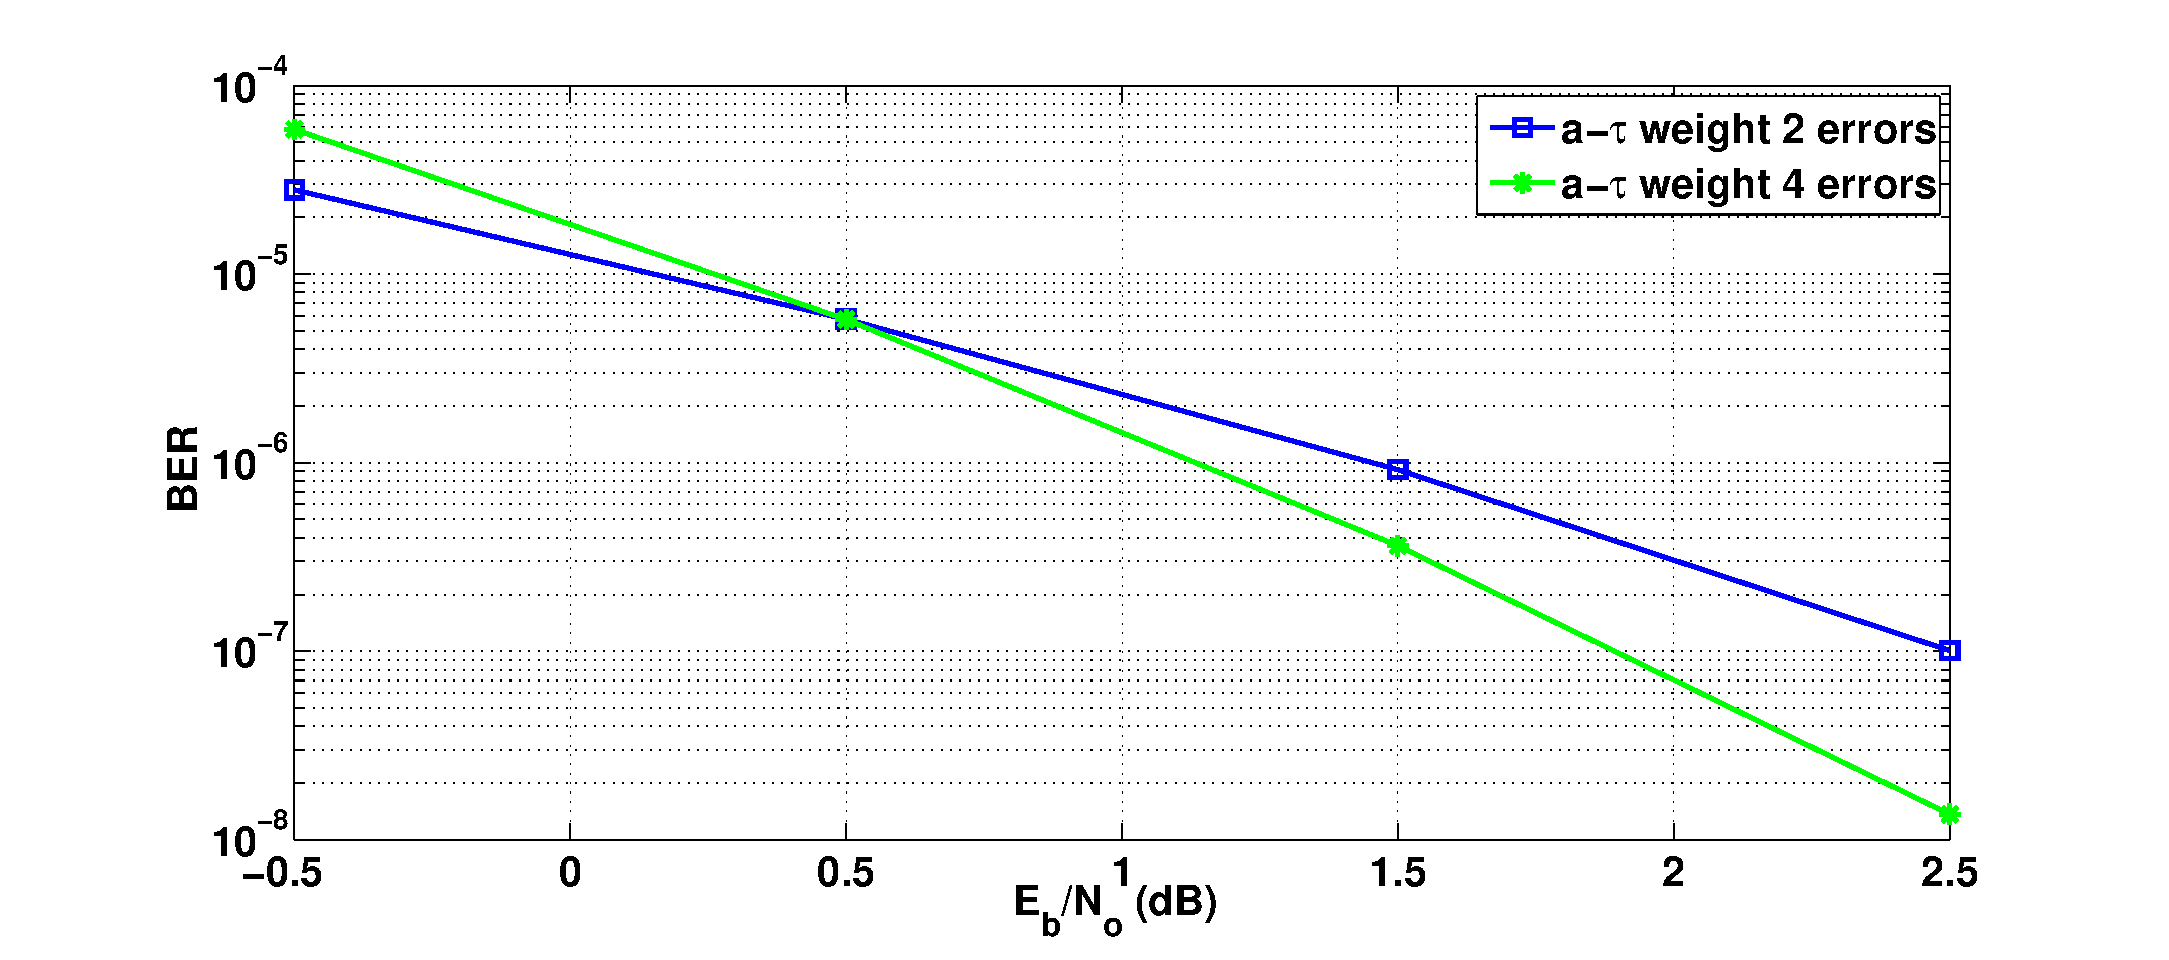
\includegraphics[width = \textwidth]{msi_D_17_s_64_N_256.eps}
		\caption{BER Upper Bound for $\Pi_{\mathit{M}|{256:(17,64)}}$.}
		\label{comp22}
		\end{figure}

\chapter{Results}
\section{Simulation Results for Interleaver Search}
Table \ref{tab1} shows the best values of $d_0$, corresponding value of$\Delta s$
 as well as  $d_{eff}$ and $N_{free,eff}$
  for an interleaver 
 of length, $N=256$ and 5/7 RSC encoder .We observe that $d_{eff}$ is the same. Since $d_0=17$ has the least
 value of $\Delta s$ and ($N_{free,eff}$), it performs the best. This is followed by
 $d_0=47$ and $d_0=31$
 %and $\frac{1 +D+ D^2+ D^3+ D^4}{1+D^4}
  %$(octal notation: 37/21).
 
 \begin{table}[h!]
\centering
\begin{tabular}{||c |c |c |c||} 
 \hline
 $d_0$ & 17 & 31 & 47 \\ [0.5ex] 
 \hline\hline
 $\Delta s$ & 64 & 128 & 64 \\ 
 \hline
  $d_{eff}$ & 38 & 38 & 38 \\ 
  \hline
  $N_{free, eff}$ & 207 & 208 & 209 \\ [1ex] 
 \hline
\end{tabular}
\caption{Best value of $d_0$,  corresponding value of $\Delta s$ 
and the value of the minimum weight codeword for
 turbo codes with $5/7$ component encoder. $N=256$}
\label{tab1}
\end{table}
Figure \ref{comp1} shows simulation results for Table 
 \ref{tab1} and the performance is as predicted with the best interleaver being $\Pi_{\mathit{M}|{256:(17,64)}}$.
\begin{figure}[h!]
\centering
		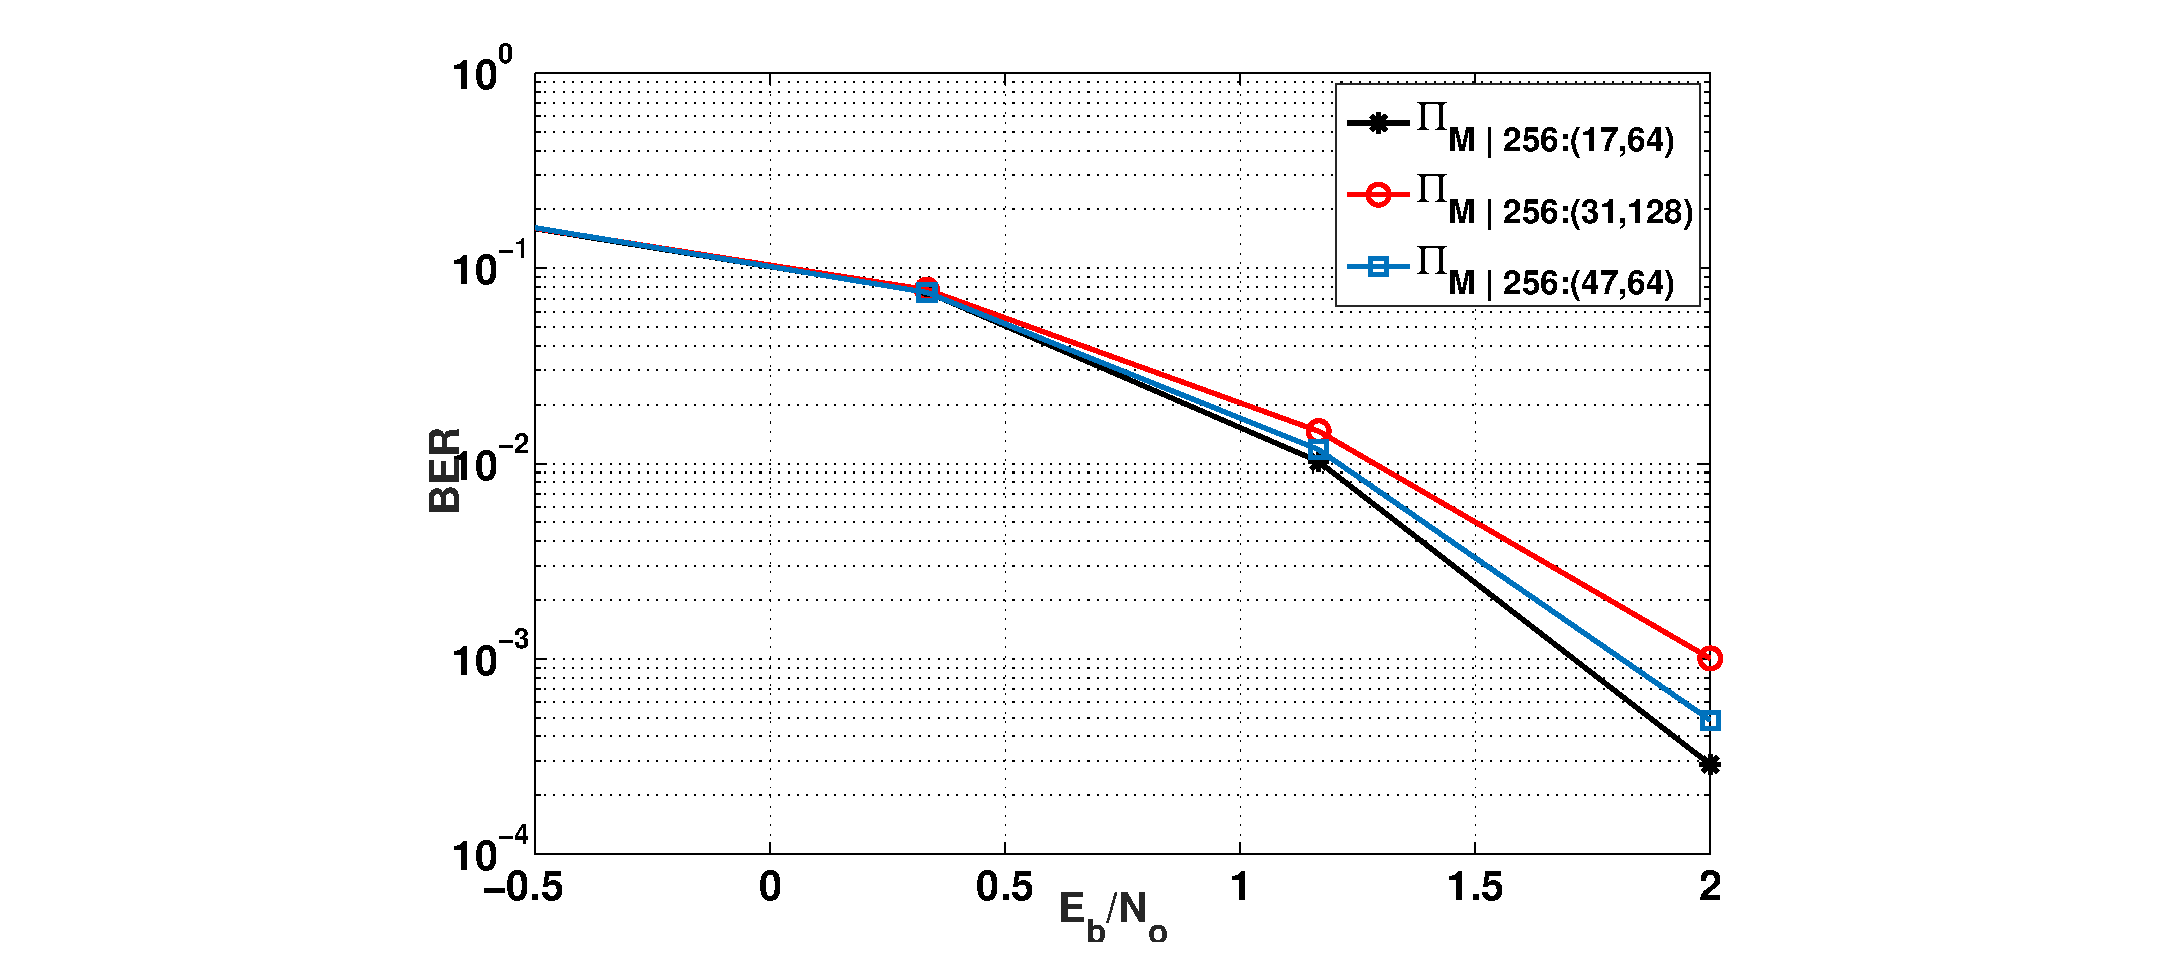
\includegraphics[width = \textwidth]{myInterleaver_(comparison_256)_5_7_3.eps}
		\caption{ Simulation Results for Table \ref{tab1}}
		\label{comp1}
		\end{figure}
		
\section{Comparison with Linear Interleavers}
Given an Interleaver of size $N=2^r$ and component code, the search for good
multi-shift interleavers is an evaluation of the best combination of $d_0$ and $\Delta s$.
 In this section, we present simulation 
results
for turbo codes designed using the multi-shift interleaver using different component
codes and compare its performance to the linear interleaver. For each simulation, 
we set the value of $d_0$ to an odd integer close to $\sqrt{N}$
and used the procedure outlined in Section \ref{secdec} to find the best value
of $\Delta s$ for the multi-shift interleaver(MSI)

 Figure (\ref{res1}) and for  Figure (\ref{res2}) are the simulation results for the 5/7 
 component code
 and the 7/5 component code with  interleaver length $N=1024$ and $D=d_0=31$. For
 the MSI, the best value of $\Delta s$ is found to be 128 and 32 for the
  $5/7$ component encoder and the
  $7/5$ component encoder respectively. We observe that in both cases
 the MSI outperforms the linear interleaver.
 \begin{figure}[h!]
\centering
		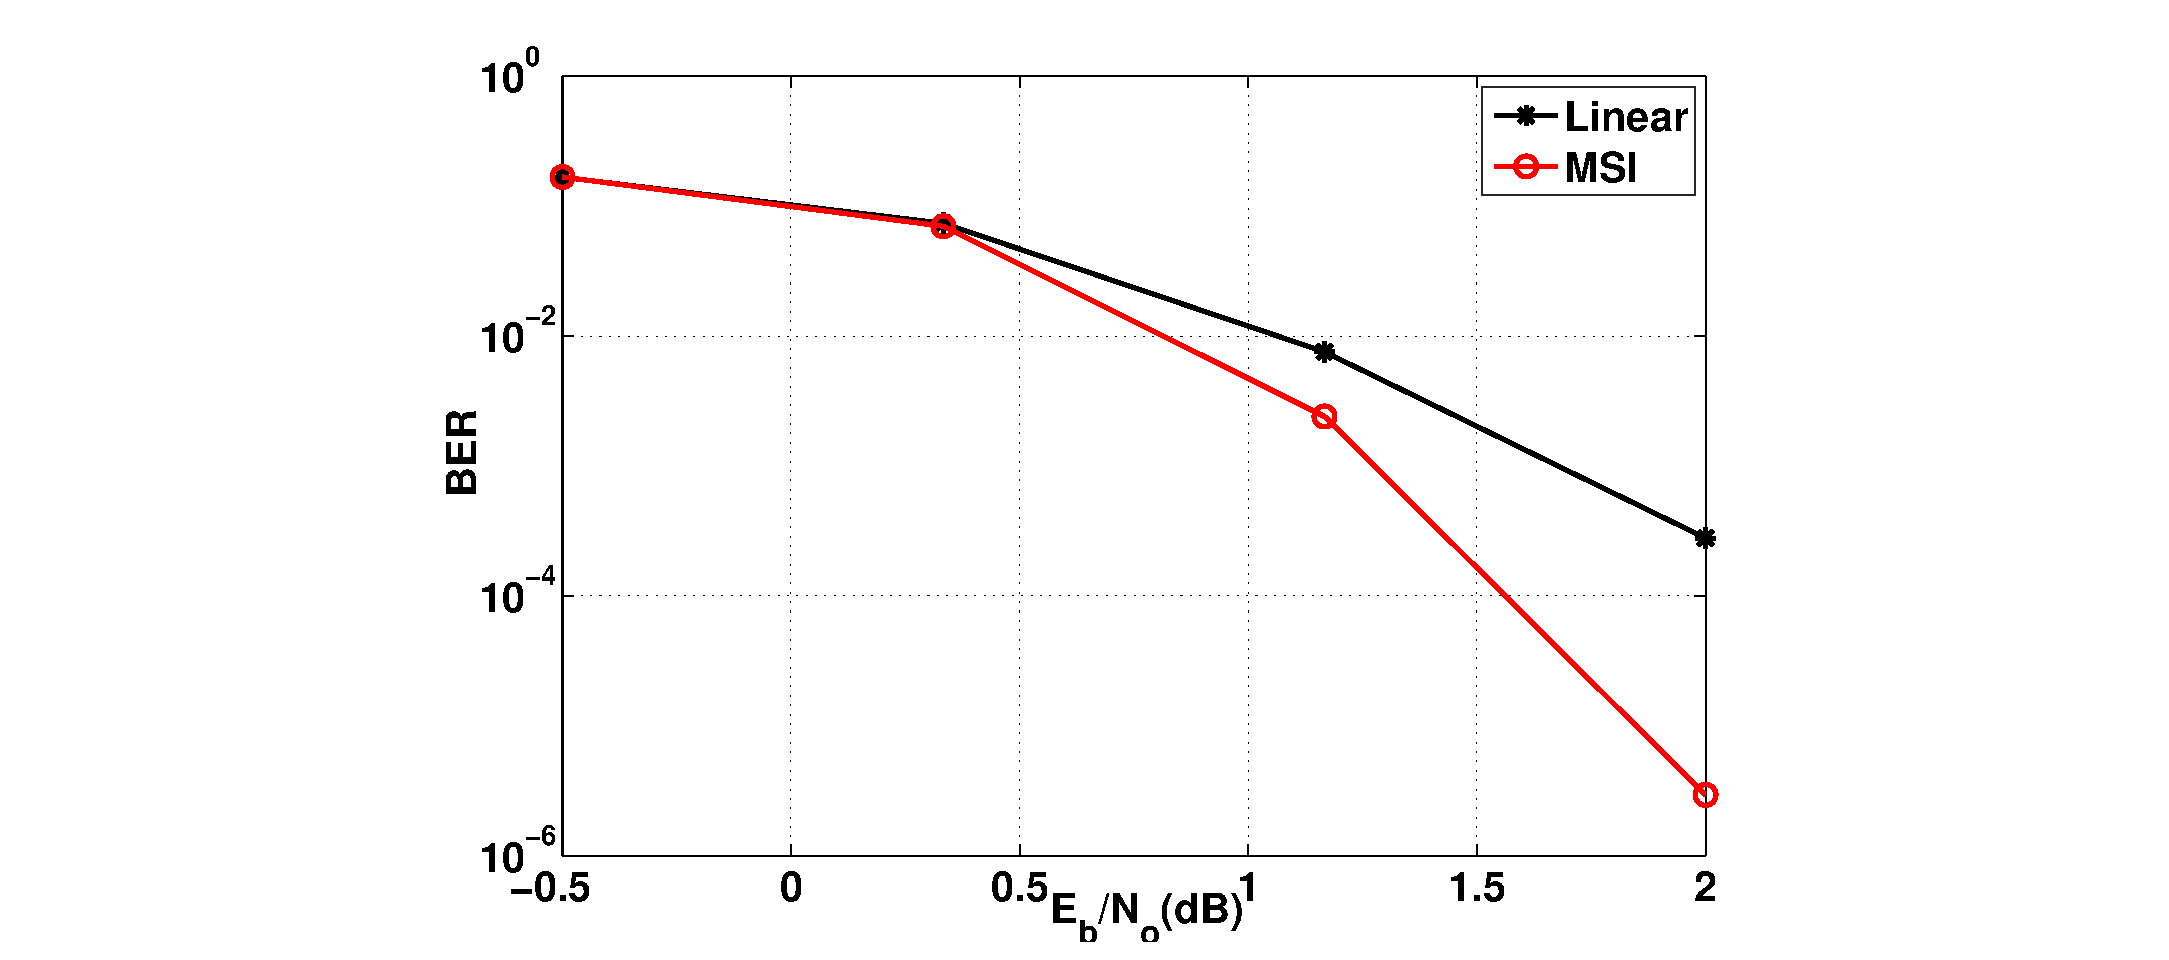
\includegraphics[width =\textwidth]{msi_linear_256_1000Frames_2.eps}
		\caption{Turbo Code with $5/7$ Component Code. $N=1024$}
		\label{res1}
		\end{figure}
		
		\begin{figure}[h!]
\centering
		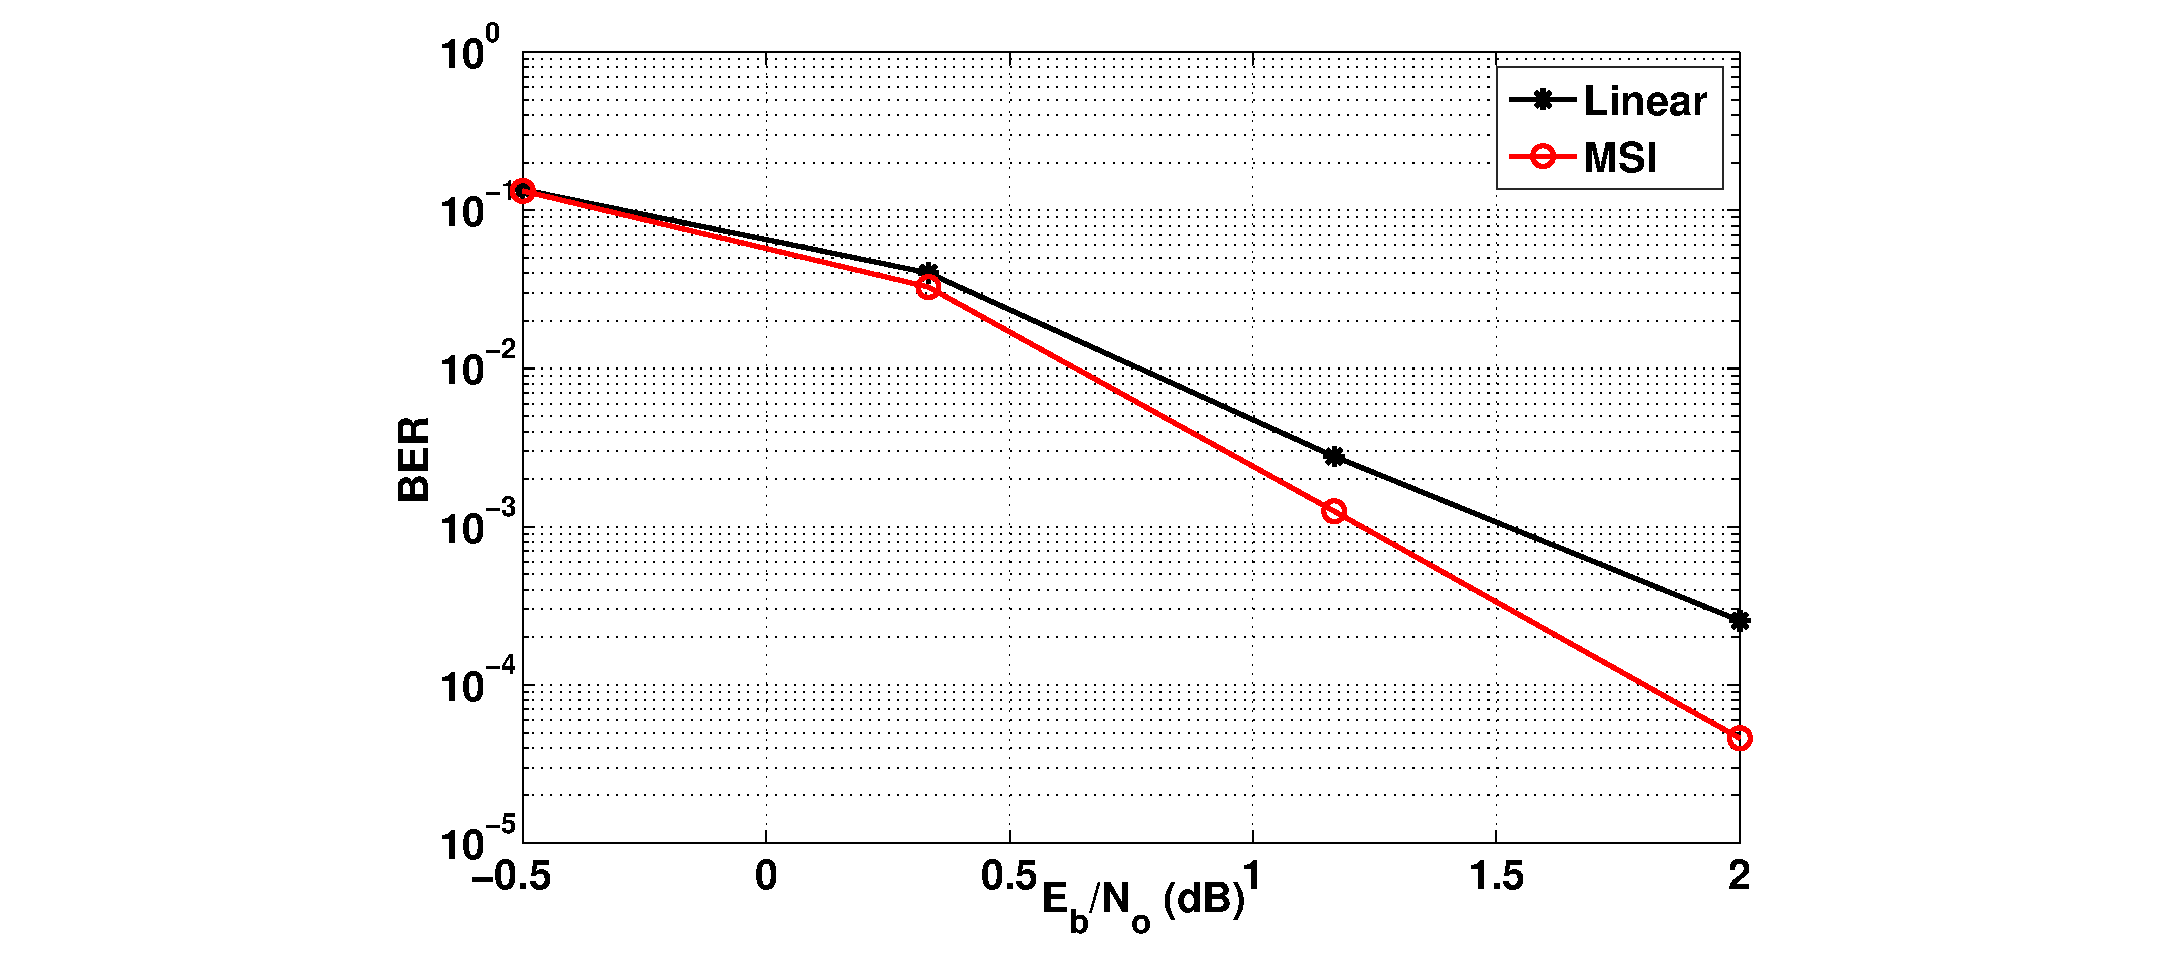
\includegraphics[width =\textwidth]{msi_linear_1024_1000_7_5Frames.eps}
		\caption{Turbo Code with $7/5$ Component Code. $N=1024$}
		\label{res2}
		\end{figure}
 In Figure (\ref{res3}), the performance of the multi-shift 
interleaver is compared with the Linear interleaver for the 
5/7 component code with interleaver length $N=16384$ and $D=d_0=127$. For the MSI
the best value of $\Delta s$ is found to be 2048. Again, the MSI outperforms the 
Linear interleaver. 


		\begin{figure}[h!]
\centering
		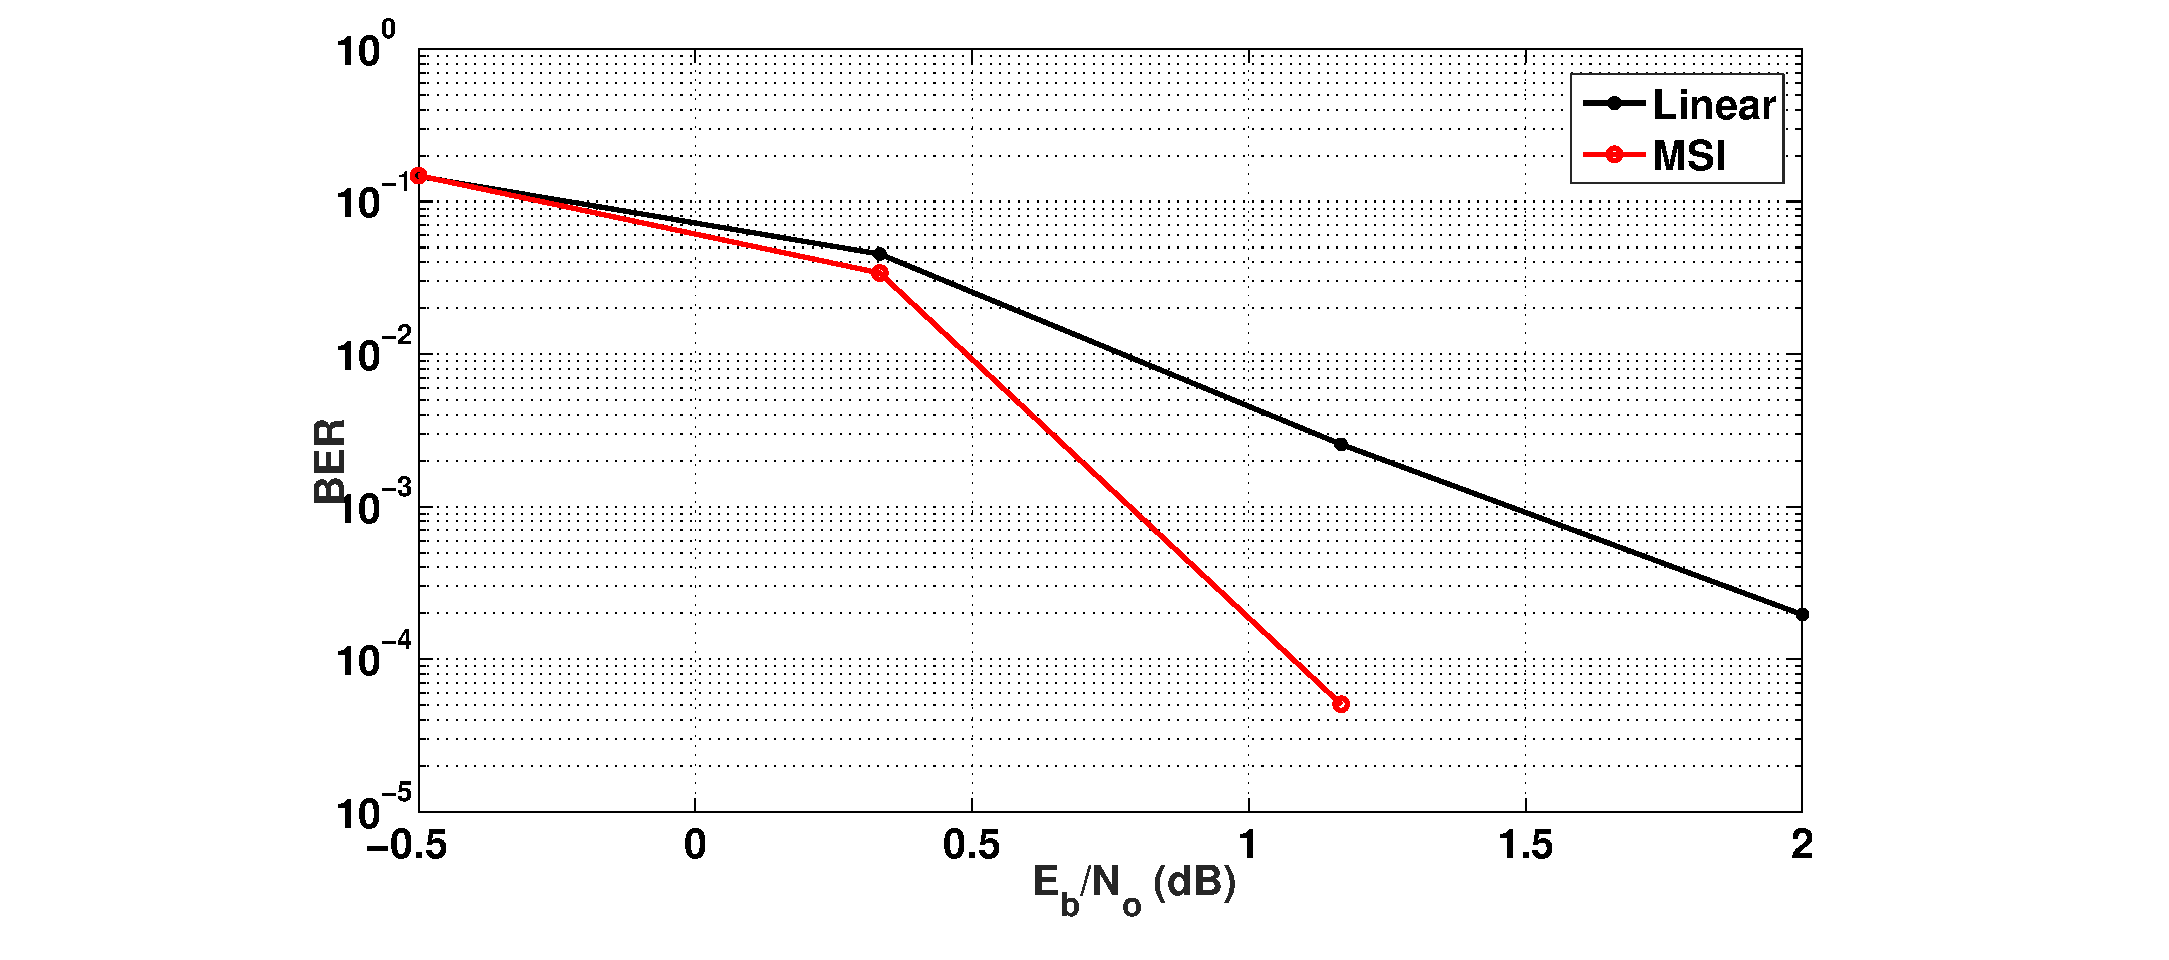
\includegraphics[width =\textwidth]{msi_linear_16384.eps}
		\caption{Turbo Code with $5/7$ Component Code. $N=16384$}
		\label{res3}
		\end{figure}


\chapter{Conclusion and Future Works}

In this research, the multi-shift interleaver was introduced. It was designed with the aim
to reduce the dominance of weight-$4 $ errors in linear interleavers although it is non-linear in nature. For a turbo code
with interleaver length $N$ and a given RSC encoder, a limited search is carried out to 
find the best value of $d_0$ and $\Delta s$ for the multi-shift interleaver. The new 
interleaver outperforms the linear interleaver for both medium and long frame sizes. 

Future work in relation to this research include the comparison of the multi-shift interleaver to the PPI and the S-random interleaver. Also we plan to find theoretical BER upper bounds for the multishift interleaver.

\chapter*{謝辞}
All glory to God who has brought me to the end of a challenging journey.I will like to thank my academic supervisor for all the assistance and direction he gave me during the research. Finally i will like to thank my labmates for their support as well.
\addcontentsline{toc}{chapter}{謝辞}
%%%%%%%%%%%%%%%%%%%%%%%%%%%%%%%%%%%%%%%%%%
\renewcommand{\bibname}{参考文献}
\addcontentsline{toc}{chapter}{参考文献}
\begin{thebibliography}{9}
\bibitem{ref1}John G. Proakis, Masoud Salehi. ''Digital Communications'', 
Fifth Edition,Chapter 8, McGraw-Hill.
\bibitem{ref2}Oscar Y. Takeshita, Member, IEEE, and Daniel J. Costello ,
''New Deterministic Interleaver Designs for Turbo Codes'',IEEE Trans. Inform. 
Theory, vol.  46,pp. 1988-2006,Nov. 2000.
\bibitem{ref3} L. C. Perez, J. Seghers, D. J. Costello, Jr.,
 ''A distance spectrum interpretation of turbo codes'', IEEE Trans. Inform. Theory, 
 vol. 42, pp. 1698-1709, Nov. 1996.
\bibitem{ref4}C. Berrou, A. Glavieux and P. Thitimajshima, 
''Near Shannon limit error-correcting coding and
decoding: Turbo codes'', Proc. Intern. Conf. Communications (ICC), Geneva, 
Switzerland, pp. 1064-
1070, May 1993.
\bibitem{ref5} Jing Sun, Oscar Y. Takeshita ''Interleavers for Turbo Codes Using 
Permutation Polynomials over Integer Rings'', IEEE Trans. Inform. Theory, vol. 51, 
pp. 101 - 119  Jan. 2005.
\bibitem{ref6} S. Benedetto and G. Montorsi, “Unveiling turbo codes: Some results
on parallel concatenated coding schemes,” IEEE Trans. Inform. Theory,
vol. 42, pp. 409 - 428, Mar. 1996.
\end{thebibliography}
\end{document}















